\chapter[Моделирование комплексов нуклеосом с белками хроматина]{Моделирование комплексов нуклеосом с белками хроматина\footnote{При подготовке данного раздела диссертации использованы следующие публикации, выполненные автором лично или в соавторстве, в которых, согласно Положению о присуждении ученых степеней в МГУ, отражены основные результаты, положения и выводы исследования: \cite{xiao_molecular_2017,gaykalova_structural_2015,valieva_large-scale_2016,gorkovets_joint_2018,bass_effect_2019,armeev_modeling_2016}.}} \label{part6_nucl_complex}

В данной главе обсуждается применение подходов интегративного моделирования для построения и анализа различных ДНК белковых комплексов, в том числе с использованием разнородных экспериментальных данных низкого информационного содержания (футпринтинг ДНК, электронная микроскопия, флюоресцентная микроскопия с использованием эффекта Ферстеровского резонансного переноса энергии). Главу предваряет введение с описанием современных представлений о структуре хроматина и некоторых подходах к его моделированию.
Материалы главы основаны на следующих статьях \cite{xiao_molecular_2017,gaykalova_structural_2015,chang_structural_2013,valieva_large-scale_2016,gorkovets_joint_2018,bass_effect_2019} и материалах конференций\cite{gorkovets_mutual_2018}.

\section{Введение}
% нужно перенести отсюда, картинки как обычно в Google draw, ссылки должны все быть https://docs.google.com/document/d/1FsWbe0d41WPVwD9ZtUDNzMLpLnfcXMClDdrN5QOls10/edit?usp=sharing
    
    

    Ключевой задачей биологии 21 века является понимание функционирования хроматина в эукариотических клетках на молекулярном уровне (см. Рисунок \ref{fig:p6_1_f1}.). Именно в хроматине происходят ключевые процессы интерпретации генетической программы клеток, определяющие их развитие и реакцию на изменение внешних условий. Комплексное решение этой задачи, понимание взаимодействия различных генетических и эпигенетических элементов в геноме (энхансеров, промотеров, инсуляторов, локусов, несущих эпигенетические модификации и т.д.) откроет дорогу к пониманию и управлению сложными регуляторными генетическими сетями, на основе которых функционируют клетки человека, животных, растений. Это в свою очередь позволит усовершенствовать методы диагностики и лечения многих заболеваний, осуществлять рациональный подход к генетическому редактированию и проектированию организмов важных с биотехнологической точки зрения.
    
    В частности известно, что многие болезни человека связаны с теми или иными нарушениями работы хроматина. Изменения в энхансер-зависимой экспрессии генов могут привести к развитию многих видов рака, а также сердечных и аутоиммунных заболеваний у людей \cite{nizovtseva_towards_2017}. Нарушение структуры хроматина и его гетерогенность, наблюдаемая при онкологических заболеваниях, позволяет раковым клеткам вырабатывать резистентность к химиотерапии, а воздействия на структуру хроматина активно рассматриваются как один из способов терапии онкозаболеваний \cite{almassalha_macrogenomic_2017}. Также например, петлеобразование в хроматине рассматривается как  лекарственная мишень для лечения бета-талласемий и серповидноклеточной анемии  \cite{krivega_chromatin_2016}.
    
\begin{figure} [H]
    \centering
    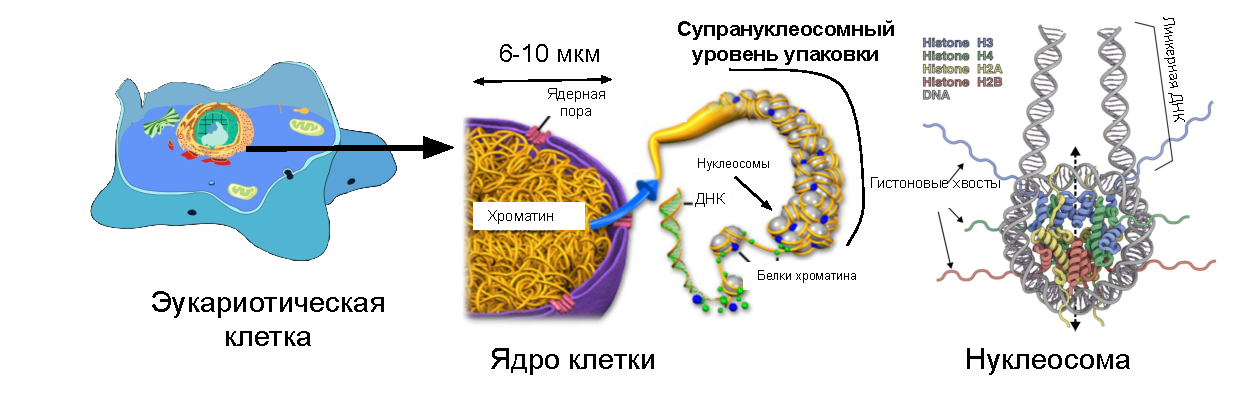
\includegraphics[width=\textwidth]{images/p6/p6_1_vved/p6_1_f1.pdf}
    \caption[От клеток к нуклеосомам.]{От клеток к нуклеосомам. Хроматин находится в ядре эукариотических клеток и включает в себя ДНК, белки и РНК. Элементарная единица упаковки ДНК - нуклеосома, комплекс из 8 гистонов (H3, H4, H2A, H2B) и около 200 пар оснований ДНК. Супрануклеосомальный уровень - уровень укладки нуклеом (от единиц до тысяч нуклеосом, от 200 до 200 000 пар оснований ДНК).}
    \label{fig:p6_1_f1}
\end{figure}
    
\begin{figure} [H]
    \centering
    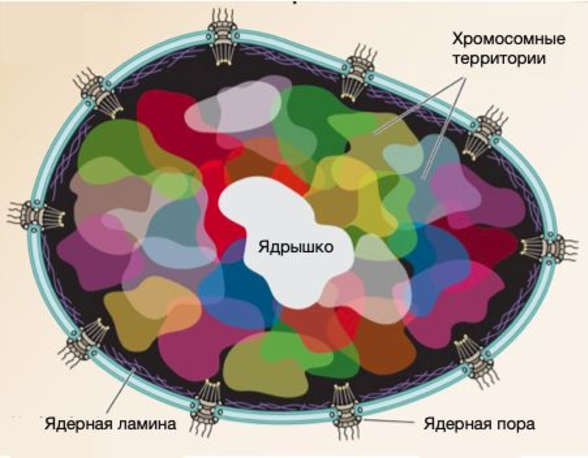
\includegraphics[width=\textwidth]{images/p6/p6_1_vved/p6_1_f2.1.pdf}
    \caption[Хромосомные территории.]{Хромосомные территории. Деконденсированные хромосомы визуализируются (флуоресцентной микроскопией) как хромосомные территории, которые таким образом являются высшим уровнем организации генома. Адаптировано из \cite{fraser_overview_2015}.}
    \label{fig:p6_1_f2.1}
\end{figure}
    
\begin{figure} [H]
    \centering
    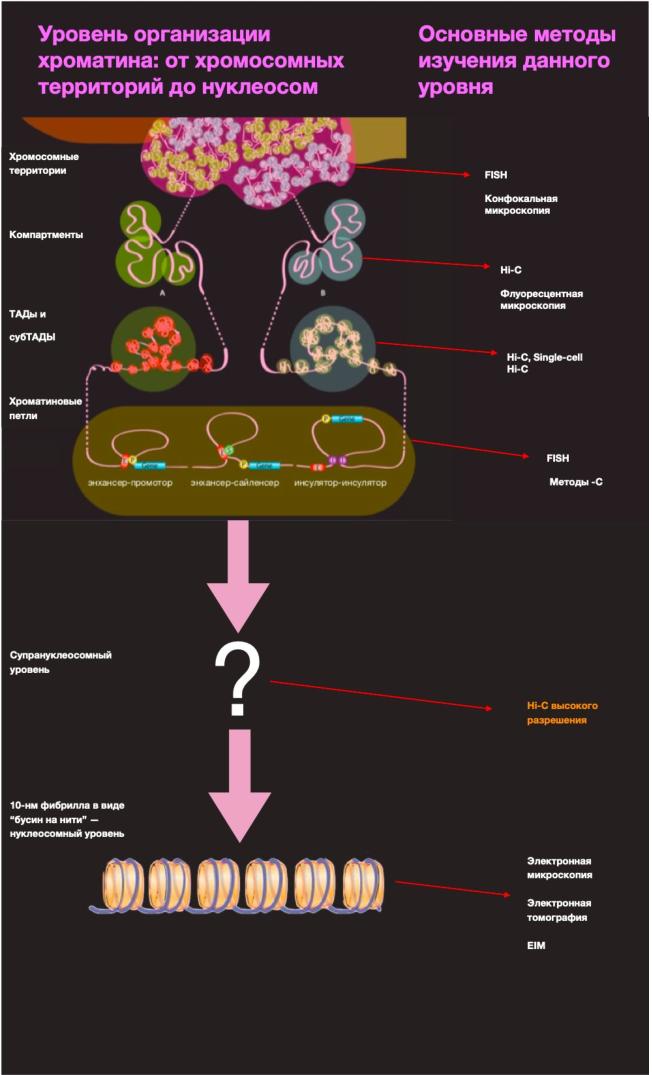
\includegraphics[width=0.5\textwidth]{images/p6/p6_1_vved/p6_1_f2.2.pdf}
    \caption[Структура хроматина и проблема ее понимания на супрануклеосомном уровне.]{Структура хроматина и проблема ее понимания на супрануклеосомном уровне. Представлены следующие за хромосомными территориями уровни организации хроматина и основные методы их обнаружения. Множественные эксперименты с использованием Hi-C говорят о существовании иерархически организованных ТАДов (Топологически ассоциированных доменов) - участков генома, локусы внутри которых чаще физически контактируют друг с другом, чем с локусами извне. Однако о физической природе ТАДов ведутся споры. Их существование пытаются связать с хорошо изученной способностью хроматина к образованию петель и наличием петель, с помощью которых регуляторные элементы генома (сайленсеры, энхансеры) взаимодействуют с регулируемыми ими промотрами генов. Также организацию хроматина на этом уровне пытаются объяснить с позиции коллоидной химии, представляя ключевым для регуляции функциональности хроматина и формирования гетерохроматина переходы между растворимым состоянием и гелеобразным состоянием (через фазу ``жидкой капли'') - модель ``разделения фаз'' \cite{larson_role_2018}.}
    \label{fig:p6_1_f2.2}
\end{figure}
    
    У человека длина всей  ДНК, содержащейся в одной клетке,  равна примерно 2 метрам (0,33 нм длина одного основания, всего около 3.1 млрд. пар оснований). При этом диаметр ядра равен примерно 6 микрометрам. То есть в ядре  ДНК сложена в 3 000 000 раз. При этом она остается функциональной -  гены способны к экспрессии. Однако, эта функциональность избирательна: в разных типах клеток для транскрипции доступны разные гены, их активность определяет уникальность клеточного типа.  Экспрессия контролируется разными способами, но одним  из наиболее важных является специфическая компактизация ДНК в хроматине. Уже с 1907 года известно \cite{gutherz_s._zur_nodate}, что хроматин бывает активным (эухроматин) и неактивным (гетерохроматин), причем последний включает в себя некоторые участки ДНК во всех клетках (конститутивный гетерохроматин), а некоторые - в зависимости от типа и состояния клетки (факультативный гетерохроматин). Эти типы, называемые также активным и неактивным компартментами хроматина, являются уровнем компактизации, следующим за наивысшим - хромосомным (в интерфазе представленном в виде хромосомных территорий, что было открыто с помощью конфокальной микроскопии и FISH -  метода визуализации индивидуальных хромосом на основе флуоресцентной гибридизации и так же хорошо обнаруживающимся с помощью обычной оптической микроскопии. В 1974 году был открыт \cite{kornberg_chromatin_1974-1} низший уровень организации хроматина - нуклеосомный: на нем ДНК наматывается на гистоновые белки, образуя структуру в виде ``бусин на нити'' — 10-нанометровую фибриллу. Этот уровень компактизации ДНК изучен хорошо, в 1997 году методами рентгеновской кристаллографии была определена структура нуклеосомы в атомарном разрешении \cite{luger_crystal_1997}, сейчас накоплено значительное количество данных о биофизике и биохимии нуклеосом и об их цепочках, которые иногда называют 10-нанометровыми фибриллами \cite{hansen_10-nm_2018}. При этом консенсуса об остальных уровнях организации хроматина в научном сообществе нет \cite{maeshima_chromatin_2014,fraser_overview_2015}. Точное представление об уровне, следующем за уровнем компартментов, отсутствует. Как 10-нанометровая фибрилла компактизуется, чтобы образовать хромосому, неизвестно. Долгое время считалось, что она образует 30-нанометровую фибриллу, которая имеет вид соленоида (одностартовая спираль) или зигзага (двустартовая спираль) в зависимости от длины линкерных участков ДНК \cite{perisic_modeling_2010}. Были получены некоторые экспериментальные данные, указывающие на существование данной структуры \cite{tremethick_higher-order_2007,rydberg_chromatin_1998}. Однако на сегодняшний день многие исследователи считают ее артефактной, не существующей \textit{in vivo}. Методы электронной томографии подтверждают существование 10-нанометровой фибриллы, но не 30-нанометровой \cite{razin_chromatin_2014,joti_chromosomes_2012}. Таким образом, организация хроматина на супрануклеосомном уровне остается неясной, поэтому ее изучение является одним из главных вызовов современной молекулярной биологии. 
    
\begin{figure} [H]
    \centering
    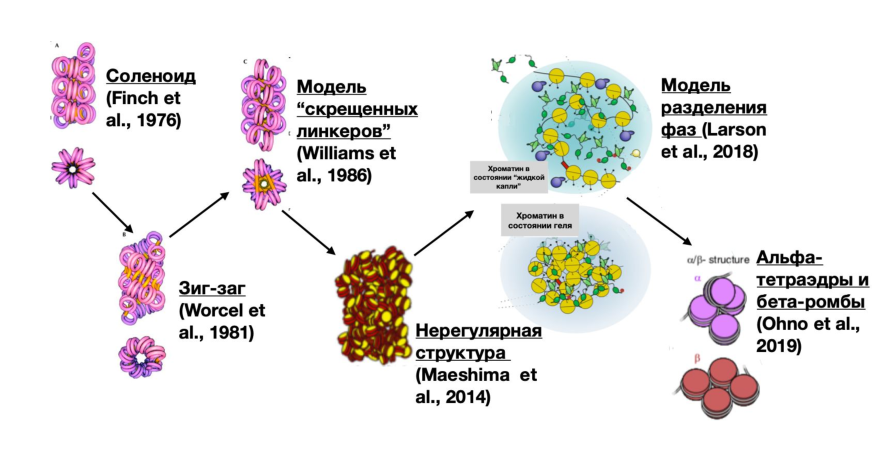
\includegraphics[width=\textwidth]{images/p6/p6_1_vved/p6_1_f3.pdf}
    \caption[О проблеме понимания организации и функционирования хроматина на супрануклеосомном уровне]{О проблеме понимания организации и функционирования хроматина на супрануклеосомном уровне. История представлений об организации супрануклеосомного уровня в хроматине. Использованы иллюстрации из: \cite{wu_variable_2007}; \cite{maeshima_chromatin_2014}; \cite{larson_role_2018}; \cite{ohno_sub-nucleosomal_2019}.}
    \label{fig:p6_1_f3}
\end{figure}
    
    Изучение трехмерной структуры генома имеет очень важное значение для исследования скоординированной работы генов и ее нарушений - например, при онкологических и наследственных заболеваниях, потому что в геноме эукариот существуют регуляторные элементы - последовательности, стимулирующие  - тогда они называются энхансерами - или ослабляющие - их название сайленсеры - экспрессию определенных генов, посредством физического контакта с их промоторами \cite{cavalli_functional_2013,nizovtseva_towards_2017}. Важно, что между регуляторным элементом и регулируемым им геном может быть большое (более мегабазы) геномное расстояние (расстояние в первичной, линейной структуре ДНК). Физический контакт происходит путем образования петли из ДНК \cite{rao_3d_2014}. Для определения наличия физического контакта между последовательностями ДНК в трехмерной структуре генома были разработаны методы семейства -С:3С,4С,5С,Hi-C \cite{fraser_overview_2015}. Эти методы основаны на химическом ``сшивании'' контактирующих в хроматине участков, фрагментации ДНК с образованием ``сшитых'' пар, лигирование фрагментов в этих парах с образованием гибридных молекул ДНК, детекция гибридных молекул (обнаружение молекулы, состоящей из последовательности А и последовательности В, говорит о физическом контакте этих последовательностей в ДНК). Метод 3С позволял оценить взаимодействие только двух участков генома друг с другом, поэтому его называли ``один против одного''. Аналогично: 4С — ``один со многими'', 5С — ``многие со многими''. Наиболее совершенным является метод Hi-C, модифицированный стадией биотинилирования гибридных молекул для обогащения ими раствора путем стрептавидинового осаждения и использованием высокоэффективного секвенирования спаренных концов \cite{lieberman-aiden_comprehensive_2009}. Hi-C - это ``все против всех''. Этот метод позволяет составить матрицу частот взаимодействий между всеми участками генома заданной длины. Метод Hi-C позволил обнаружить следующий за компартментами уровень компактизации хроматина - Топологически ассоциированные домены (ТАДы) - регионы ДНК, в пределах которых взаимодействие участков друг с другом происходит чаще, чем с участками из других регионов\cite{dixon_topological_2012}.
    
    Хотя ТАДы проявляются как определенный паттерн на матрице взаимодействий, их физическая природы неясна \cite{pal_hi-c_2019}. Существуют две основные концепции относительно нее. Первая - DNA loop extrusion (``выпетливания ДНК'') предполагает возникновение на участке ДНК, ограниченном сайтами связывания белка CTCF, петли, расширяющейся со временем до этих сайтов \cite{sanborn_chromatin_2015}. В разных клетках петля в пределах сайтов связывания CTCF находится на разных стадиях расширения - соответственно в разных клетках рядом оказываются разные участки ДНК, что на матрице Hi-C отображается как ТАД. Слабость этой гипотезы в том, что она считает ТАДы популяционным феноменом, в то время как интрахромосомные ТАДы (в отличие от интерхромосомных) и хроматиновые глобулы, считающиеся соответствующими ТАДам, обнаруживаются и в отдельных клетках \cite{nagano_single-cell_2013}. Другая гипотеза утверждает, что ТАДы - это особые хроматиновые домены, возникающие в клетках из-за физического взаимодействия между нуклеосомами в неактивном хроматине \cite{ulianov_active_2016}. Эта гипотеза тоже имеет недостаток - она не объясняет расположения сайтов связывания CTCF на границах ТАДов. Таким образом очевидно, что необходимо продолжать исследования структуры хроматина и на уровне ТАДов. Так как ТАДы отчасти ``фрактальны'' -  содержат внутри себя вложенные друг в друга ТАДы меньших размеров - изучение хроматина даже на супрануклеосомном уровне может помочь понять структуру всей иерархии ТАДов \cite{phillips-cremins_architectural_2013,norton_detecting_2018}. 
    
    Для исследований регуляторной функции хроматина необходимо понимать его супрануклеосомальную организацию. Так, обеспечение коммуникации между энхансером и промотером, которые могут располагаться на расстояниях до нескольких сотен килобаз, обеспечивается за счет образования петель. Энхансеры - элементы, которые обеспечивают транскрипционную активацию подавляющего большинства генов человека и в значительной степени определяют состояние хроматина вблизи промоторных областей. Эпигенетическими метками активных энхансеров явяются, в частности, H3K27ac, H3K4me1, H3K27me3, и гистоновые варианты H3.3 и H2A.Z. К меткам промотеров относятся: H3K4me3 и H3K27ac \cite{nizovtseva_towards_2017}. 
    
    Исследования энхансеров затрудняются их различиями в последовательности ДНК. Большинство промотеров ассоциировано с 1 энхансером, в то время как 25\% промотеров - с двумя или больше в разные моменты времени. Известно более миллиона энхансеров, а одновременно активны порядка тысячи энхансеров. 
    
    Изменения в энхансер-зависимой экспрессии генов могут привести к развитию многих видов рака, а также сердечных и аутоиммунных заболеваний у людей. К изменению активности энхансеров в онкологических заболеваниях  приводит изменение копийности энхансеров, структурные перестройки генома, изменяющие таргетный ген энхансера и точечные мутации или индели, которые влияют на связывание с транскрипциоными факторами и образовывают новые энхансеры или наоборот, разрушают инсуляторы \cite{sur_role_2016}. 
    
    Актуальной проблемой в области лечения онкологии, в части в химиотерапии, является развитие резистентности к лекарственным агентам. Так, в работе \cite{almassalha_macrogenomic_2017} было показано, что использование агентов, влияющих на внутриядерные изменения плотности упаковки хроматина, приводит к уменьшению транскрипционной гетерогенности и, соответственно, к предотвращению возникновения химиорезистентности. 
    
 \subsection{О прогрессе методов структурной биологии в изучении супрануклеосомной организации} 

    Кристаллическая структура коровой частицы нуклеосомы (гистоны H3, H4, H2A, H2B и 145-147 пар оснований ДНК) с атомистическим разрешением была получена в 1997 году \cite{luger_crystal_1997} (Рисунок \ref{fig:p6_1_f4}). Позднее стало очевидно, что данная структура является лишь некоторым компактным вариантом, который удовлетворяет условиями кристаллической упаковки, а сама нуклеосома достаточно динамична. Несмотря на биохимические данные о динамичности нуклеосом, получения различных вариантов ее структуры в динамике стало возможным лишь недавно благодаря успехам криоэлектронной микроскопии \cite{bilokapic_structural_2018}. Также благодаря криоэлектронной микроскопии в последние годы получены разнообразные структуры нуклеосом с белками хроматина, в частности структура нуклеосомы при прохождении РНК-полимеразы \cite{ehara_structural_2019}, структуры нуклеосом с различными ремоделлерами (белковыми комплексами перемещающими нуклеосомы или заменяющими гистоны) \cite{farnung_nucleosomechd1_2017,li_mechanism_2019,yan_structures_2019}.
    
    Важной вехой явилось определения структуры хроматосомы - комплекса нуклеосомы с линкерным гистоном H1 \cite{bednar_structure_2017}.
    
    Применение криоЭМ к определению структуры нуклеосомальных фибрилл также проводилось. Были получены структуры нуклеосмных фибрилл с и без гистона H1 \cite{song_cryo-em_2014}. Однако, данные фибриллы, состоящие из 12 нуклеосом, находящихся на равном расстоянии друг от друга, были приготовлены искусственно. Поэтому значение данной структуры для понимания биологических процессов ставится под сомнение.

\begin{figure} [H]
    \centering
    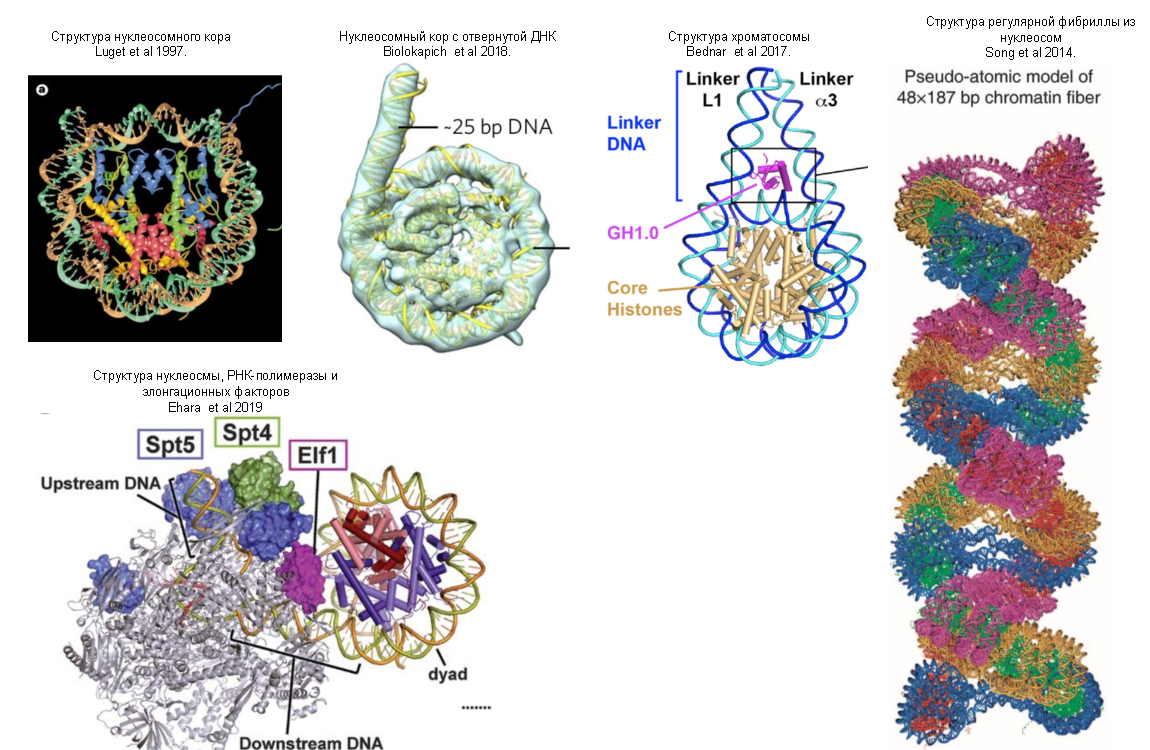
\includegraphics[width=\textwidth]{images/p6/p6_1_vved/p6_1_f4.pdf}
    \caption{Различные структуры нуклеосом, их комплексов и фибрилл из нуклеосом, полученные в последнее время методами структурной биологии.}
    \label{fig:p6_1_f4}
\end{figure}
    
    
    
    
    
    
    
    
    
    
    
    
    
    
    
    
    
    
    
    
    
    
    
    
    
    
    
    
    
    
    
    
    
    
    
    
    
    
    
    
    
    
    
    
    
    
    
    
    
    
    
    
    
    
    
    
    
    
    
    
    
    
    
    
    
    
    
    
    
    


\section{Комплексы нуклеосомы и РНК-полимеразы}
\textit{Текст данного раздела основан на статьях \cite{gaykalova_structural_2015,chang_structural_2013}}.
%здесь нужно будет куски текста и картинки  из двух статей перевести. Ссылки нужно будет добавить - их нет в зотеро многих. В описании картинок - не забывать добавить из какой они статьи - ссылку.
%materials/part6_2_nucl_pol/pnas2015 и nar2014

\subsection{Введение}
%2S pnas2015 - желтое выделение.
    Транскрипция РНК-полимеразы II (Pol II) индуцирует обширное ремоделирование хроматина, сопровождающееся ковалентными модификациями гистонов и их обменом (см. напр. \cite{smolle_resetting_2013,das_histone_2013,zentner_regulation_2013}). В то же время, гистоны вытесняются только из высокотранскрибируемых генов \cite{kristjuhan_evidence_2004,schwabish_evidence_2004,lee_evidence_2004}; таким образом, Pol II обычно встречается с нуклеосомами во время транскрипции каждого участка ДНК длиной $\sim$200 пар оснований. Остающиеся нуклеосомы на транскрибируемых генах образуют два типа барьеров для транскрипции Pol II \cite{das_histone_2013,weber_nucleosomes_2014}. Во-первых, каждая нуклеосома представляет собой барьер, на котором Pol II приостанавливается после транскрипции 40–50 п.н. от границы нуклеосомы проксимальной к промотор. Во-вторых, намного выше барьер образован первой (+1) транскрибированной нуклеосомой, по крайней мере в дрозофилы \cite{weber_nucleosomes_2014}; в этом случае Pol II останавливается на нуклеосомной границе. Остановившаяся Pol II обнаружена на многих генах: от 15\% до более чем 50\% генов у мух и человека соответственно \cite{guenther_chromatin_2007,muse_rna_2007,zeitlinger_rna_2007}. В во многих случаях остановившаяся Pol II была картирована вместе с хорошо расположенной +1 нуклеосомой. Предполагается, что эта +1 нуклеосома может через паузирование влиять на общий уровень экспрессии генов \cite{weber_nucleosomes_2014,mavrich_nucleosome_2008}. 
    
    Данные \textit{in vitro} экспериментов установили, что даже одна нуклеосома может образовывать высокий барьер первого типа для транскрипции Pol II \cite{brown_activator-dependent_1996,izban_transcription_1991,bondarenko_nucleosomes_2006,kireeva_nature_2005,kulaeva_mechanism_2009,hall_high_2009} и что факторы транскрипции, шапероны гистонов, модификации гистонов и т.д. необходимы Pol II  для преодоления этого барьера \cite{bondarenko_nucleosomes_2006,kireeva_nature_2005,brown_disruption_1997,izban_factor-stimulated_1992,hsieh_histone_2013,kulaeva_rna_2010,kim_human_2010,guermah_synergistic_2006,carey_rsc_2006,bintu_nucleosomal_2012,jin_synergistic_2010}. Сильный барьер образуется после транскрипции 40–50 п.н. за границей нуклеосомы [область +(40–50)], является нуклеосомно-специфичным, специфичным для Pol II и был описан для всех проанализированных организмов, от дрожжей до человека \cite{izban_transcription_1991,bondarenko_nucleosomes_2006,kireeva_nature_2005}. Таким образом +40–50 нуклеосомный барьер является ``универсальным'' признаком транскрипции через хроматин с помощью Pol II и может использоваться для регуляции экспрессии на уровне элонгации транскрипта \cite{bondarenko_nucleosomes_2006}. На любой последовательности ДНК, барьер формируется в различных положениях внутри региона +(40–50)  \cite{bondarenko_nucleosomes_2006}.

\subsection{Создание моделей комплекса в положении активного центра +49 (нулевая петля)}
%2S дать желтый текст из nar2014, картинки основного текста и таблицу тоже
    Наши предыдущие исследования выявили элонгационный комплекс +49 (ЭК+49, 49 п.н. от промотор-проксимальной границы нуклеосомы), содержащий нулевую петлю, в качестве ключевого интермедиата, который помогает нуклеосомам выживать во время транскрипции \cite{kulaeva_mechanism_2009}. В данной работе мы смоделировали комплекс ЭК+49 путем докирования структуры высокого разрешения элонгационного комплекса дрожжевой полимеразы II  на нуклеосому с 601 хорошо позиционирующей последовательностью ДНК \cite{vasudevan_crystal_2010,kettenberger_complete_2004} (Рисунок \ref{fig:p6_2_n2014_f1}).
    
    ЭК+49 имеет следующие свойства (Рисунок \ref{fig:p6_2_n2014_f1}): (i) Основная часть молекулы Pol II обращена в раствор и не имеет стерических конфликтов с гистонами нуклеосомного кора, (ii) Изгиб ДНК на $90^{\circ}$, присутствующий в ЭК, обращен к октамеру и позволяет формировать нулевую петлю, (iii) контакты ДНК-гистоны на участком ДНК длиной $\sim$20 п.н. за ЭК стабилизируют нулевую петлю, (iv) вытеснение 50 п.н. с конца нуклеосомы дистального к промотору снижает размер области ДНК, взаимодействующей с гистонами перед ферментом с $\sim$100 до $\leq$50 п.н. Это, вероятно, способствует дальнейшему разворачиванию ДНК с октамера впереди от Pol II и транскрипции через нуклеосому \cite{kulaeva_mechanism_2009}. (v) Отрицательно заряженная область на поверхности Pol II (предполагаемая последовательность, стабилизирующая нулевую петлю, область ZLS - zero-loop-stabilizing sequence) находится в непосредственной близости к положительно заряженной области октамера гистонов и, таким образом, может стабилизировать нулевую-петлю и способствовать выживанию нуклеосом во время транскрипции.
    
\subsection{Выявление отрицательно заряженных регионов на предполагаемых
гистон-взаимодействующих поверхностях Pol II}
    
    Используя модель ЭК+49 (рис. \ref{fig:p6_2_n2014_f1}), были идентифицированы предполагаемая взаимодействующая с Pol II поверхность на октамере гистонов и три взаимодействующие с гистоном поверхности Pol II (рис. \ref{fig:p6_2_n2014_f2}A). Все взаимодействующие с гистонами поверхности заряжены отрицательно и локализуется на самой крупной субъединице дрожжевой Pol II (yRpb1, регионы 1–3, рис. \ref{fig:p6_2_n2014_f2}А). Для дальнейшей оценки возможной роли предполагаемых областей ZLS на Pol II во время транскрипции через хроматин было оценено их присутствие и сохранение в различных структурно связанных эукариотических и прокариотические РНК-полимеразах  (Таблица \ref{tab:p6_n2014_t1}). РНКП \textit{Escherichia coli}, которая использует механизм транскрипции типа Pol II через хроматин \cite{walter_bacterial_2003} не была включен в это исследование, потому что структуры с высоким разрешением этого фермента пока не получена. Последовательности областей 2 и 3 ZLS является консервативными с более, чем 50\% идентичностью, у мультисубъединичных прокариотических РНКП \textit{T. thermophilus} и \textit{T. aquaticus} ( структурно сходных с Pol II \cite{vassylyev_structural_2007,zhang_crystal_1999}), а как область 1 консервативна только в эукариотических РНКП. Гомологичных последовательностей в односубъединичный РНКП бактериофага Т7 не было обнаружено.
    
    Предполагается, чтобы чистый отрицательный заряд последовательности ZLS может быть важен для стабилизации нулевой петли и эффективного выживания нуклеосомы в ходе транскрипции \cite{kulaeva_mechanism_2009}. В соответствии с этим предположением области ZLS отрицательно заряжены в дрожжевой Pol II (Рисунок \ref{fig:p6_2_n2014_f2}A), которая не смещает нуклеосомы во время транскрипция \cite{kireeva_nucleosome_2002,walter_bacterial_2003}. Области ZLS Pol II человека также отрицательно заряжены, и поэтому ожидается, что Pol II человека также сохраняет нуклеосомную структуры во время транскрипции. Это предложение согласуется с наблюдаемыми сходными паттернами сильной нуклеосомной паузы, которые характерны для Pol II человека и дрожжей \cite{bondarenko_nucleosomes_2006}.
    
    Напротив, отрицательные заряды областей ZLS не сохранились в других проанализированных прокариотических РНКП (из \textit{T. thermophilus} и \textit{T. aquaticus}) (Рисунок \ref{fig:p6_2_n2014_f2}Б и Таблица \ref{tab:p6_n2014_t1}).
    
    Хотя предполагаемая взаимодействующая с гистонами поверхность РНКП \textit{T. thermophilus}  имеет некоторые регионы с локальным отрицательным зарядом (рис. \ref{fig:p6_2_n2014_f2}Б), в данном регионе нет суммарного положительного заряда. Данные показывают, что чистый отрицательный заряд внутри взаимодействующего с гистоном поверхности этих РНКП положительно коррелирует с вероятность выживания нуклеосом при транскрипции. Кроме того, расстояние между областями ZLS и поверхность октамера гистонов в среднем на $\sim$5\AA больше для РНКП \textit{T. thermophilus}, чем у дрожжевой Pol II. Более низкий полный отрицательный заряд областей ZLS и больше расстояние между РНКП и октамером гистонов, вероятно, уменьшает силу взаимодействия между РНКП и гистонами. Соответственно, РНКП, которые имеют более низкий полный отрицательный заряд области ZLS, как ожидается, формируют менее стабильный комплекс нулевой петли в положении ЭК +49. Поскольку стабильная нулевая петля, вероятно, необходима для выживания нуклеосом, ожидается, что эффективность выживаемости будет ниже во время транскрипции РНКП \textit{T. thermophilus} и \textit{T. aquaticus} по сравнению с Pol II. Поскольку стабильная нулевая петля также приводит нуклеосомной паузе в области +45 \cite{hsieh_histone_2010}, уменьшение паузирования в положении +45 также ожидается во время транскрипции этими РНКП. Чтобы проверить эти предсказания модели, эксперименты по транскрипции на идентичных ДНК и нуклеосомных матрицах были проведены с помощью РНКП \textit{T. thermophilus} и \textit{T. aquaticus}.
    
\begin{figure} [H]
    \centering
    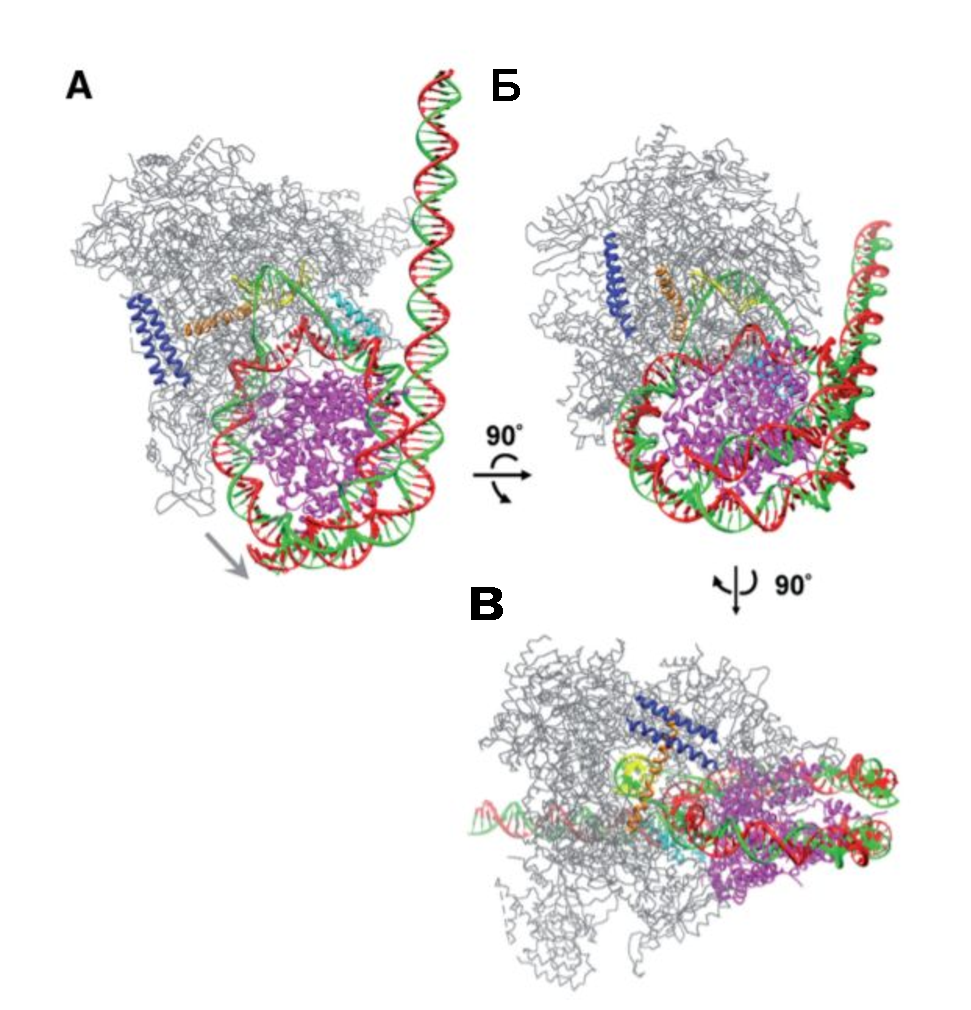
\includegraphics{images/p6/p6_2/p6_2_nar2014_f1.pdf}
    \caption[Модель ЭК+49 (нулевая петля) с дрожжевой Pol II]{Модель ЭК+49 (нулевая петля) с дрожжевой Pol II. (A) Структуры нуклеосомы и комплекса элонгации Pol II дрожжей с активным сайтом в позиции +49 [PDB 3LZ0 и 1Y1W соответственно \cite{vasudevan_crystal_2010,kettenberger_complete_2004}] были объединены с использованием подхода докинга. Чтобы позволить формирование небольшой внутринуклеосомной петли ДНК, содержащей транскрибирующую Pol II, промотор-дистальная область нуклеосомной ДНК длиной 50 п.н. была отмотана от октамера \cite{kulaeva_mechanism_2009}. Октамер нуклеосомы изображен пурпурным. Матричная цепь ДНК, нематричная цепь ДНК и цепи РНК изображены зеленым, красным и желтым, соответственно. Мостовая спираль (bridge), зажим (clamp), C-терминальная двойная спираль (coiled coil) и остальная часть молекулы Pol II показаны оранжевым, голубым, синим и серым, соответственно. Серая стрелка указывает направление транскрипции. (Б) Структура была повернута на $\sim 90^{\circ}$ вокруг горизонтальной оси. (В) Затем структура была повернута на 90 $^{\circ}$ вокруг вертикальной оси.}
    \label{fig:p6_2_n2014_f1}
\end{figure}
   
\begin{figure} [H]
    \centering
    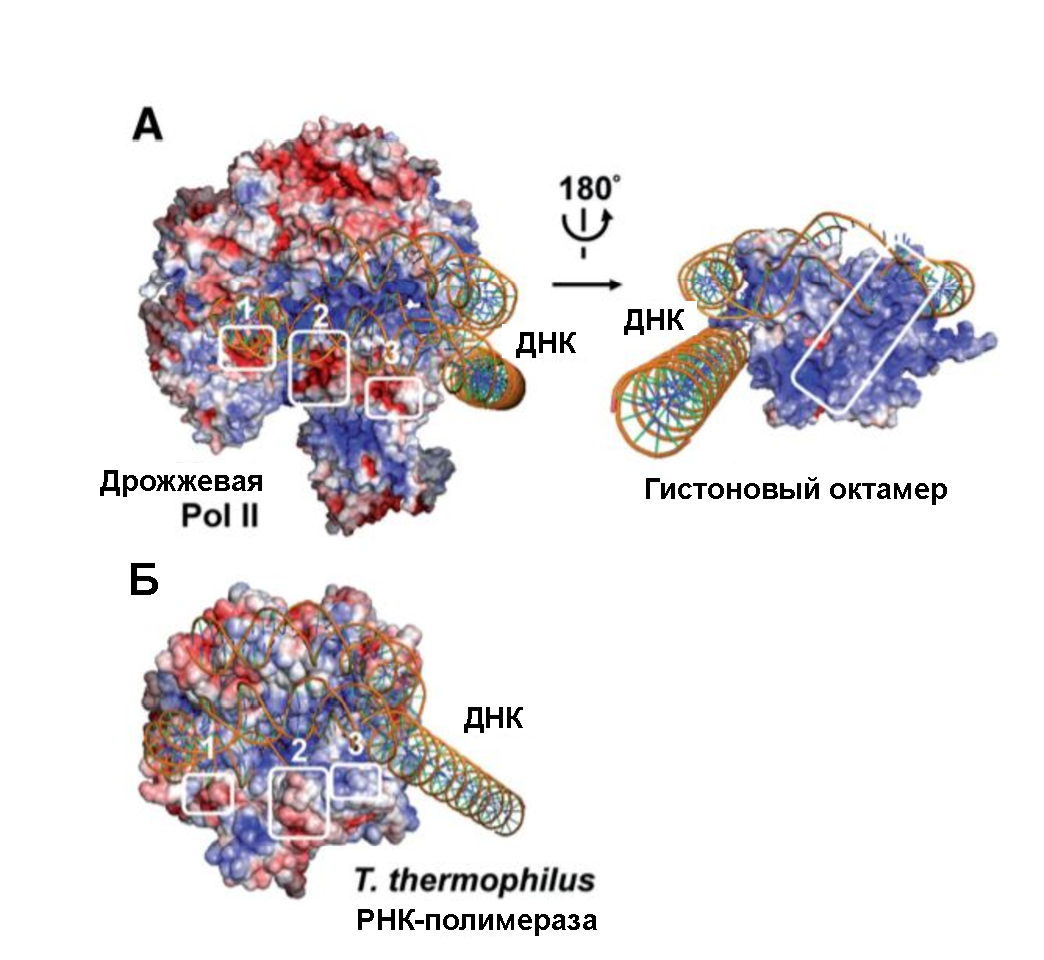
\includegraphics{images/p6/p6_2/p6_2_nar2014_f2.pdf}
    \caption[Отрицательно заряженная поверхность Pol II может стабилизировать интермедиат нулевой петли посредством взаимодействия с гистоновым октамером]{Отрицательно заряженная поверхность Pol II может стабилизировать интермедиат нулевой петли посредством взаимодействия с гистоновым октамером. (А) Предполагаемые взаимодействующие с гистонами молекулярные поверхности дрожжевой Pol II. Слева: Три идентифицированные поверхности на большой субъединице Rpb1 дрожжевой Pol II внутри ЭК+49 (смоделирована как на Рисунке \ref{fig:p6_2_n2014_f1}), взаимодействующие с октамером гистонов (не показан), показаны белыми квадратами (области 1–3). Справа: контактирующая поверхность на октамере гистонов (повернут на $180^{\circ}$ вокруг вертикальной оси). Самый темный синий и самый темный красный цвет обозначает электростатический потенциал 5 кТ/е и -5 кТл/е, соответственно. ДНК показана желтым. (Б) Молекулярные поверхности РНКП \textit{T. thermophilus} (PDB ID 2O5I) в гипотетической модели комплекса ЭК+49 окрашены по величине электростатического потенциала (октамер гистонов не показан). Области 1–3 гомологичны контактирующим с гистоном поверхностям Pol II (Figure \ref{fig:p6_2_n2014_f2}A).}
    \label{fig:p6_2_n2014_f2}
\end{figure}

\begin{table}
\begin{threeparttable} [h!]
    \centering
    \begin{tabularx}{\textwidth}{|X|X|X|X|X|X|}
\hline
        Фермент & Виды & Заряд ZLS области\tnote{a} & Нулевая петля при +49 & Высота +45 барьера & Выживание нуклеосом \\
\hline
        Pol II (RPB1) & \textit{H. sapiens} & -8 & ND & $+++++$\tnote{b} & ND \\
        Pol II (Rpb1) & \textit{S. cerevisiae} & -15 & $+$\tnote{c} & $+++++$\tnote{b} & $+++++$\tnote{d} \\
        РНКП ($\beta'$) & \textit{T. thermophilus} & +1 & ND & $+$\tnote{e} & ND \\
        РНКП ($\beta'$) & \textit{T. aquaticus} & +1 & $-$\tnote{e} & $+$\tnote{e} & - \\

\hline
    \end{tabularx}
\begin{tablenotes}
    \item[a] Полные заряд гомологичной области 1434–1450 ZLS субъединицы Rpb1 дрожжевой Pol II.
    \item[b]  Ссылка \cite{bondarenko_nucleosomes_2006}.
    \item[c]  Ссылка \cite{kulaeva_mechanism_2009}.
    \item[d]  Ссылка \cite{walter_bacterial_2003}.
    \item[t]  Эта работа.
     
   \end{tablenotes}
\end{threeparttable}
    \caption{Корреляция между присутствием отрицательно заряженных областей на обращенной к октамеру поверхности РНКП, высотой нуклеосомного барьера и выживаемостью нуклеосом во время транскрипции}
    \label{tab:p6_n2014_t1}
\end{table}

\subsection{Более высокий отрицательный заряд области ZLS коррелирует с более сильным барьером +45 и более эффективной выживаемостью нуклеосом при транскрипции}
    
    Данные о чистом заряде региона ZLS, силе барьера +45 нуклеосомного паузирования и судьбы нуклеосом во время транскрипции различными РНКП просуммирована в Таблице \ref{tab:p6_n2014_t1}. Наличие более высокого отрицательного заряда область ZLS положительно коррелирует с формированием ключевого промежуточного продукта, который сильно способствует выживанию нуклеосом (нулевая петля в положении +49), с более сильным паузированием в области +45 и более эффективным выживанием нуклеосом во время транскрипции.
    
    В целом данные свидетельствуют о том, что присутствие и полный заряд области ZLS частично определяет структуру ключевого интермедиата, сформированного в позиции +49, а в в свою очередь, судьбу нуклеосом при транскрипции. Когда ZLS область присутствует и отрицательно заряжена (например, у Pol II человка или дрожжей), нуклеосомное паузирование в положении +45 является сильным, нулевая петля образуется в положении +49 и нуклеосомы эффективно выживают во время транскрипции. Когда регион ZLS присутствует, но не содержит отрицательного заряда (например, в РНКП \textit{T. thermophilus} и \textit{T. aquaticus}), нуклеосомная пауза в +45 положении слабая, нулевая петля не образуется, и нуклеосомы теряются во время транскрипции.
    
    
    
\subsubsection{Дискуссия и сравнение с экспериментами} %not edited
%2S дать фиолетовый текст из nar2014, картинки основного текста
    
    В нашей работе роль отрицательно заряженной области на поверхности Pol II (области ZLS) во время транскрипции через хроматин было оценено с использованием компьютерного моделирования и экспериментального анализа механизма транскрипция через хроматин различными РНКП. Вычислительное моделирование показало, что в комплексе элонгации, определяющем выживаемость нуклеосом во время транскрипции (ЭК+49), три области ZLS находятся в непосредственной близости к положительно заряженной области октамера гистонов и таким образом могут стабилизировать нулевую-петлю и облегчать нуклеосомную выживаемость при транскрипции (рисунки \ref{fig:p6_2_n2014_f1} и \ref{fig:p6_2_n2014_f2}). Анализ транскрипции РНКП \textit{T. thermophilus} и \textit{T. aquaticus}, у которых есть незаряженные области ZLS, предполагает, что в этом случае нуклеосомная пауза +45 слабая, нулевая-петля не образуется, и нуклеосомы теряются во время транскрипции. Напротив, транскрипция Pol II, имеющая отрицательно заряженные области ZLS, приводит к сильной нуклеосомной паузе в +45 положении, образовании нулевой-петли и выживаемости нуклеосом \cite{kireeva_nucleosome_2002,kulaeva_mechanism_2009,bondarenko_nucleosomes_2006}. Сила +45 паузы частично определяется отрицательным зарядом в области ZLS Pol II. Таким образом свойства (в частности, заряд) области ZLS диктуют все ключевые параметры механизма транскрипции через нуклеосому.
    
    Как может наличие и заряд ZLS региона влиять на эти множественные аспекты транскрипции через хроматин? Ранее мы предположили, чтобы регион ZLS может влиять на структуру/стабильность ключевого интермедиата, содержащего нулевую-петлю (ЭК+49), образующегося во время транскрипции через нуклеосому \cite{kulaeva_mechanism_2009}. Это промежуточное состояние, в свою очередь, как ожидалось будет играть связывающую роль между паузированием в +45 положении и эффективным выживанием нуклеосом во время транскрипции \cite{hsieh_histone_2010}. В соответствии с этим предположением наши текущие данные свидетельствуют в пользу того, что РНКП у которых отсутствует заряд в области ZLS или сама область не сталкиваются с сильным нуклеосомным барьером, не образуют нулевые-петли и не могут поддерживать эффективное выживание нуклеосом.
    
    Основываясь на наших данных, мы предлагаем следующую модель, объясняющую наблюдаемую связь между +45 паузой, образование нулевой петли и судьбой нуклеосом. По мере того как разные РНКП входят в нуклеосому и подходят к области +45 (комплекс 1), они образуют нулевую-петлю с разной эффективностью. В частности, дрожжевой Pol II образует нулевую петлю (комплекс 2) с высокой эффективностью \cite{kulaeva_mechanism_2009}, отчасти потому, что ее ZLS-область заряжена отрицательно и стабилизирует нулевую петлю за счет взаимодействия с положительно заряженной поверхностью октамера гистонов. Формирование нулевой петли вызывает медленное раскручивание ДНК перед ферментом (комплекс 3) - то есть сопровождается сильной нуклеосомной паузой. ДНК позади РНКП повторно оборачивается вокруг октамера гистонов и нуклеосома восстанавливается в исходном положении \cite{kulaeva_mechanism_2009}. Напротив, во время транскрипции РНКП \textit{T. thermophilus} и \textit{T. aquaticus} с незаряженными ZLS областями нуклевая петля (если образуется) нестабильна (комплекс 2'). Таким образом, транскрипция сопровождается лишь незначительной нуклеосомной паузой и смещением гистонового октамера при дальнейшей транскрипции через нуклеосому \cite{walz_sequence_1975}. Таким образом, структуры ключевых промежуточных продуктов образующиеся во время транскрипции через +45 область нуклеосомной ДНК, вероятно, обуславливают множество аспектов транскрипции через хроматин, включая нуклеосомную паузу и судьбу гистонов при транскрипции. Присутствие и заряд региона ZLS вряд ли будет единственным фактором, влияющим на результат транскрипции через хроматин. Таким образом, расстояние между областями ZLS и октамером гистонов в ЭК+49, вероятно, важно для стабильность нулевой петли.
    
    Отрицательно заряженная область 2 ZLS дрожжевого Pol II  локализована в свитч-2 домене и, вероятно, важна для разделения нитей ДНК при транскрипции \cite{kettenberger_complete_2004}. Она также локализована в кислотном домене, который влияет на активацию транскрипции, активность Pol II дрожжей и важен для нормального роста клеток \cite{xiao_highly_1994}. Наши исследования предполагают дополнительную важную функцию области 2 ZLS - определение скорости прохождения РНКП через нуклеосому и судьбу нуклеосом при транскрипции в хроматине. Эта функция особенно важна для эукариотических Pol II: в данном случае консервативный отрицательно заряженная область ZLS, скорее всего, способствует выживанию нуклеосом и поддержанию гистоновых меток во время транскрипции.
    
% \begin{figure} [H]
%     \centering
%     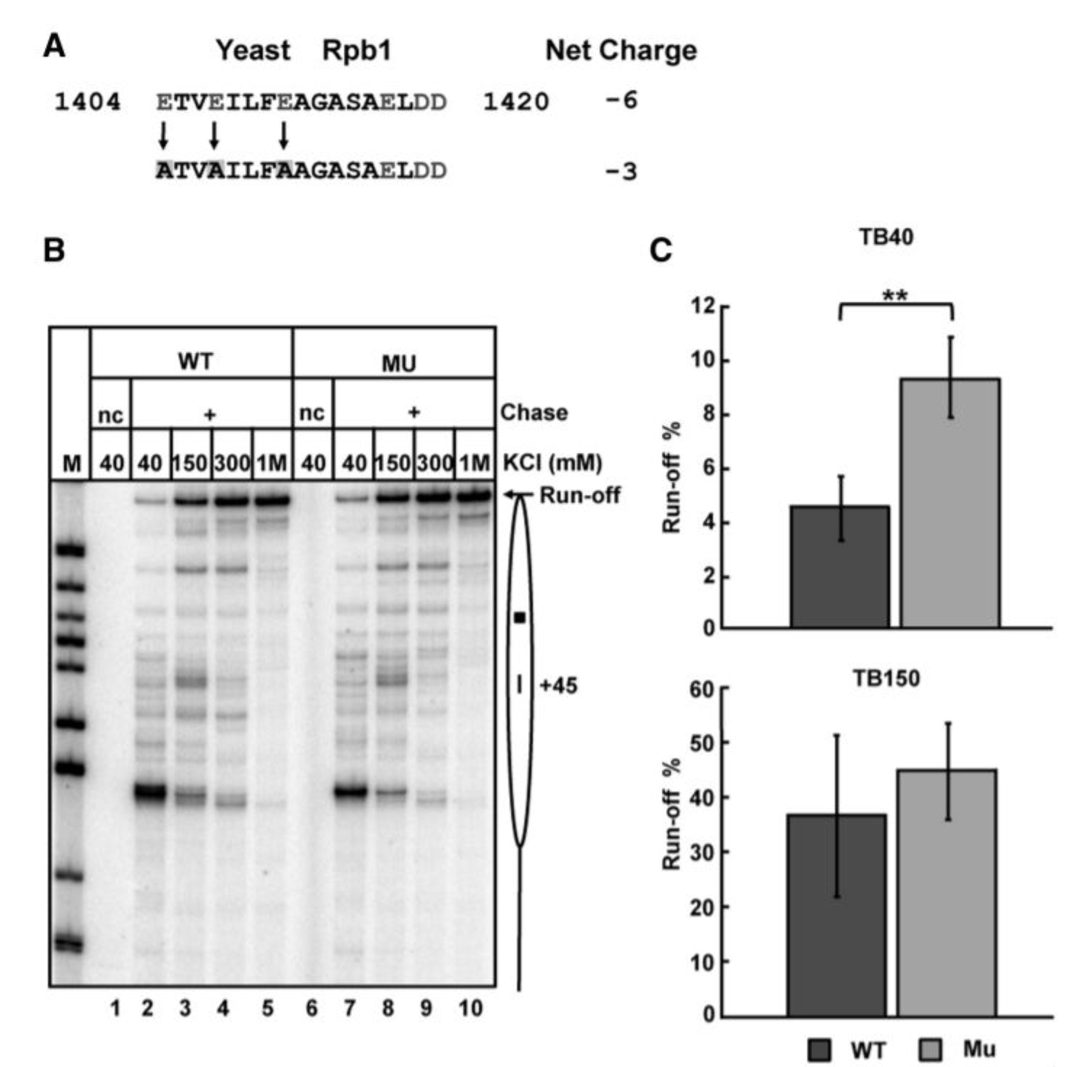
\includegraphics{images/p6/p6_2/p6_2_nar2014_f6.pdf}
%     \caption{MU Pol II, имеющий более низкий отрицательный заряд взаимодействующей с гистонами поверхности, встречает более низкий нуклеосомный барьер. (A) Стратегия Pol II мутагенез. Три аминокислоты Glu субъединицы yRpb1 в положениях 1404, 1407 и 1411 одновременно были преобразованы в Ala (отмечены желтым квадратов), изменяя чистый заряд области 2 ZLS с –6 до –3. Отрицательно заряженные аминокислоты выделены жирным красным цветом. (Б) Транскрипция 603 нуклеосомные матрицы с помощью WT и MU yPol II при указанных концентрациях KCl. nc означает отсутствие погони. РНК с импульсной меткой анализировали с помощью денатурирующий PAGE. Другие обозначения такие же, как на рисунке \ref{fig:p6_2_n2014_f4}. (В) Количественное определение транскриптов, полученных при 40 мМ KCl и 150 мМ KCl WT. или Mu yPol II (Рисунок \ref{fig:p6_2_n2014_f7}Б). Показаны средние значения из трех экспериментов и стандартные отклонения (** означает значение P <0,01).}
%     \label{fig:p6_2_n2014_f6}
% \end{figure}
    
\begin{figure} [H]
    \centering
    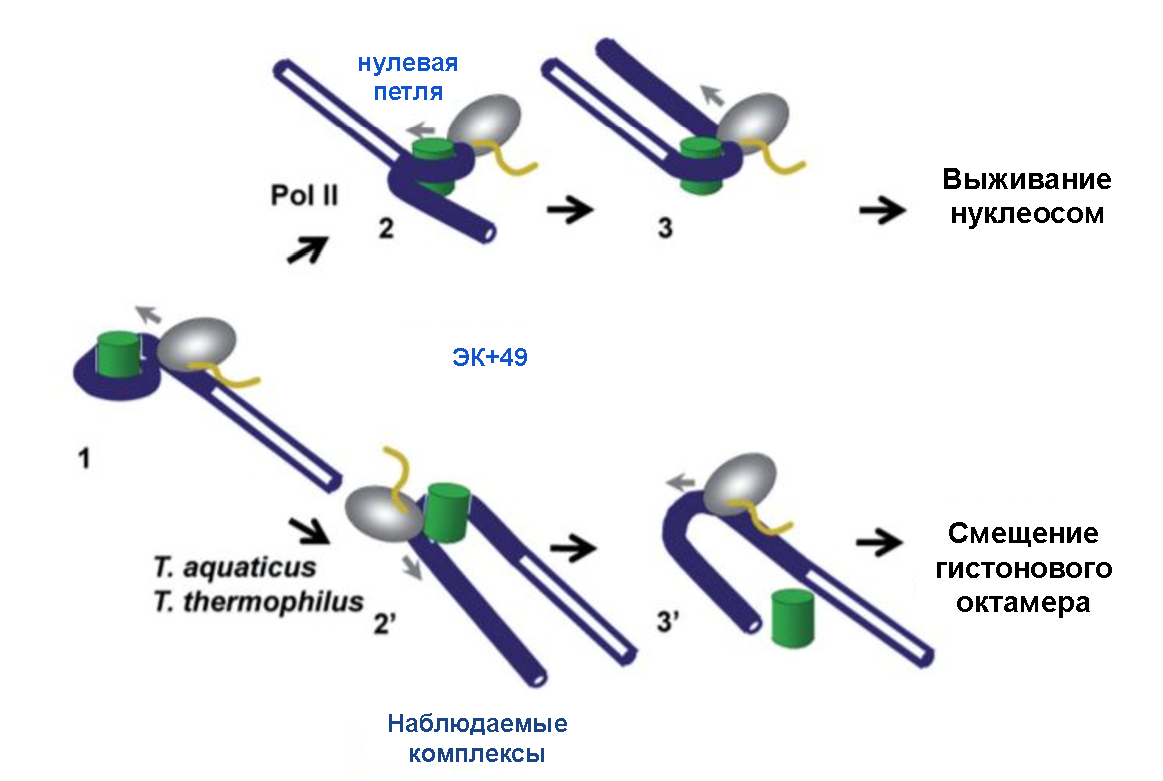
\includegraphics[width=\textwidth]{images/p6/p6_2/p6_2_nar2014_f7.pdf}
    \caption[Предлагаемые механизмы транскрипции через нуклеосому разными РНКП.]{Предлагаемые механизмы транскрипции через нуклеосому разными РНКП. Мы предлагаем, чтобы общий отрицательный заряд на поверхность РНКП, которая обращена к октамеру гистонов, частично обуславливает структуру важного промежуточного комплекса (ЭК+49). Более подробное описание см. в тексте.}
    \label{fig:p6_2_n2014_f7}
\end{figure}
    
    
    
    
    
    
    
    
    
    
\subsubsection{Методы}
%2S зеленый кусок текста из nar2014
\subsubsection{Моделирование Pol II в позиции +49 в нуклеосоме и анализ структурных особенностей моделируемых комплексов}
    
    Модель была построена с использованием программа UCSF Chimera (\url{http://www.cgl.ucsf.edu/chimera/}) \cite{pettersen_ucsf_2004} за счет объединения структуры коровой частицы нуклеосомы на основе 601 последовательности [PDB ID 3LZ0 \cite{vasudevan_crystal_2010}] со структурой элонгационного комплекса дрожжей Pol II [PDB ID 1Y1W \cite{kettenberger_complete_2004}]. Веб-сервер 3D-DART использовался для восстановления конформации ДНК \cite{van_dijk_3d-dart_2009}. Остальные подходы следовали описанию в опубликованной статье \cite{kulaeva_mechanism_2009}. ЭК+49 \textit{T. thermophilus} был построен путем наложения кристаллической структуры РНКП [PDB ID: 2O5I \cite{vassylyev_structural_2007}] на модель Pol II ЭК+ 49. Молекулярные электростатические поверхности белков рассчитывали с помощью APBS \cite{baker_electrostatics_2001} и отображали с помощью PyMOL (\url{http://www.pymol.org}). Расстояния между отрицательно заряженной поверхность Pol II и октамером гистонов, а также вовлеченные аминокислотные остатки также были идентифицированы в PyMOL. Все белковые последовательности РНКП в этой статьи были взяты из базы данные RefSeq NCBI (NP\_000928.1, NP\_010141.1, NP\_418415.1, YP\_145078.1 и CAB65466.3) (\url{http://www.ncbi.nlm.nih.gov/guide/}). Последователности различных РНКП были выровнены с помощью NCBI Blast (\url{http://blast.ncbi.nlm.nih.gov}).
    
    











\subsection{Создание моделей комплекса полимеразы и нуклеосомы в положении активного центра +42}
%2S pnas2015 - зеленый текст
%(картинки только основные, не сапплемент, кроме s5 и s8 - которые нужно дать.)
%дать синий текст
\subsubsection{Экспериментальные данные}
    Эксперименты проводились с использованием мононуклеосомных матриц, которые повторяют многие важные аспекты транскрипции PolII в хроматине \textit{in vivo} \cite{kulaeva_rna_2010,kireeva_nucleosome_2002,hsieh_histone_2010}. Механизм образования нуклеосомного барьера при транскрипции изучен с использованием 601 и 603 мононуклеосом, которые содержат ДНК последовательность с полярным барьером для транскрипции  (PBS) и образуют очень сильный нуклеосомный барьер в одна из двух транскрипционных ориентаций (непермиссивная ориентация) \cite{bondarenko_nucleosomes_2006,kulaeva_mechanism_2009,gaykalova_polar_2011}. Матрицы ДНК были разработаны так, чтобы Pol II останавливалась в положениях -41 и -5 (на 41 или 5 п.н. выше промоторно-проксимальной границы нуклеосомы) при наличие различных частичных комбинаций нуклеотид трифосфатов. Pol II спонтанно останавливается во время транскрипции непермиссивной нуклеосомы 601 при 150 мМ KCl на +46 и +48 позиции. Остановка обратима, так как Pol II может транскрибировать всю матрицу после дестабилизации гистонового октамера в 1M KCl.
    
    Состояние Pol II после встречи с высоким нуклеосомный барьером изучалось с помощью 601-ой ДНК матрицы, которая представляет собой самый сильный нуклеосомный барьер для транскрипции Pol II \cite{bondarenko_nucleosomes_2006}. Pol II был спонтанно останавливалась в позиции +46 и +48 на 601-нуклеосомной матрице.
    
    Для определения положения активного центра Pol II комплексы +46 и +48 инкубировали в присутствии факторов элонгации транскрипции IIS (TFIIS). TFIIS - это фактор транскрипции, который сильно облегчает расщепление РНК в активном центре Pol II после ее отката (backtracking) \cite{fish_promoting_2002}. Инкубация комплексов элонгации с TFIIS приводили к образованию гомогенной РНК длиной 42 неуклеотида, что указывает на то, что оба комплекса откатываются на 4 или 6 п.н. до положения +42. Нуклеосомные комплексы +42, +46 и +48 остаются полностью функциональными и могут реактивироваться после удаления нуклеосом в присутствие 1 М KCl. Таким образом, когда Pol II сталкивается с сильным нуклеосомным барьером, она останавливается и возвращается назад на 4–6 п.н. Возврат может привести к образованию щели в комплексе между Pol II и нуклеосомой, если нуклеосомная ДНК не закручивается обратно на поверхность октамера.
    
    Вращательная ориентация Pol II в позиции +42 после отката несовместима с формированием нулевой петли \cite{kulaeva_mechanism_2009}. Поэтому мы ожидали, что нуклеосомная ДНК будет отмотана от октамера перед комплексом +42.

    Доступность нуклеосомной ДНК в комплексе +42 была анализировали с помощью анализа чувствительности к рестриктазам. Нуклеосома сильно защищает ДНК от переваривания рестрикционными ферментами \cite{polach_restriction_1999}. В ЭК+42 только сайт AflIII расположен выше активного центра (но не Сайты RsaI или MfeI, расположенные ниже по течению) чувствительен к расщеплению. Таким образом, ДНК в комплексе +42 отворачивается от октамер выше этой позиции, но тесно связана с гистонами ниже активного центра фермента.
    
    \subsubsection{Моделирование структуры комплекса Pol II с нуклеосомами и ее анализ}
   Структура комплекса +42 РНКП с нуклеосомой была определена с помощью электронной микроскопии в режиме одиночного анализ частиц. ЭК+42 имеет суммарную молекулярную массу около 545 кДа, что затрудняет их наблюдение в криоЭМ. Поэтому контраст изображения был увеличен с помощью негативного контрастирования уранилацетатом. Всего 8 500 частиц комплекса ЭК+42 были проанализированы. Финальная структура содержит более крупную (диаметром около 20 нм) и меньшую (около 14 нм в диаметре) плотность. Детальные структурные особенности комплекса не могут быть разрешены при полученном разрешении в 22\AA. 
   
   Поэтому нами были применены алгоритмы интегративного моделирования для восстановления структуры комплекса.
 Для моделирования ЭК+42, рентгеновская структура элонгационного комплекса РНКП \textit{Thermus thermophilus}  \cite{vassylyev_structural_2007}  была совмещена с рентгеновской структурой  нуклеосомы \cite{davey_solvent_2002} за счет удлинения нижележащего дуплекса ДНК с сегментом прямой B-ДНК и соединения его с различными соответствующими положениями вдоль нуклеосомной ДНК, соблюдая правильную геометрию ДНК и химических связей. Далее РНКП \textit{T. thermophilus} была заменена структурой РНКП \textit{E. coli} \cite{zuo_mechanism_2013} посредством суперпозиции структур поскольку структуры двух ферментов очень похожи. Моделирование проводили с помощью UCSF  Chimera \cite{pettersen_ucsf_2004} и программы Nucleic Acid Builder (NAB) \cite{bomble_multiscale_2008}. Полученный ансамбль моделей автоматически вписывался в экспериментально полученную карту 
 электронной плотности с помощью утилиты Chimera EM (атомистическая модель была преобразована в расчетную карту электронной плотности с разрешением 30\AA{}  и проводился обширный поиск с 40 различными пробными стартовыми пространственными положениями). Лучшая модель была выбрана на основе максимальной кросскорреляции электронных плотностей. В полученной модели активный центр РНКП находится в позиции +42; нижестоящий дуплекс ДНК входит в нуклеосому в положении +71 (за 3 п.н. до положения оси диады). Полученная модель представлена на рисунке \ref{fig:p6_2_pnas_f6}.
 Наконец, структура дрожжевого элонгационного комплекса Pol II (PDB ID 1Y1W) \cite{kettenberger_complete_2004} была наложена на структуру РНКП \textit{E. coli} для получения Pol II +42 элонгационного комплекса.
   
   \begin{figure} [H]
    \centering
    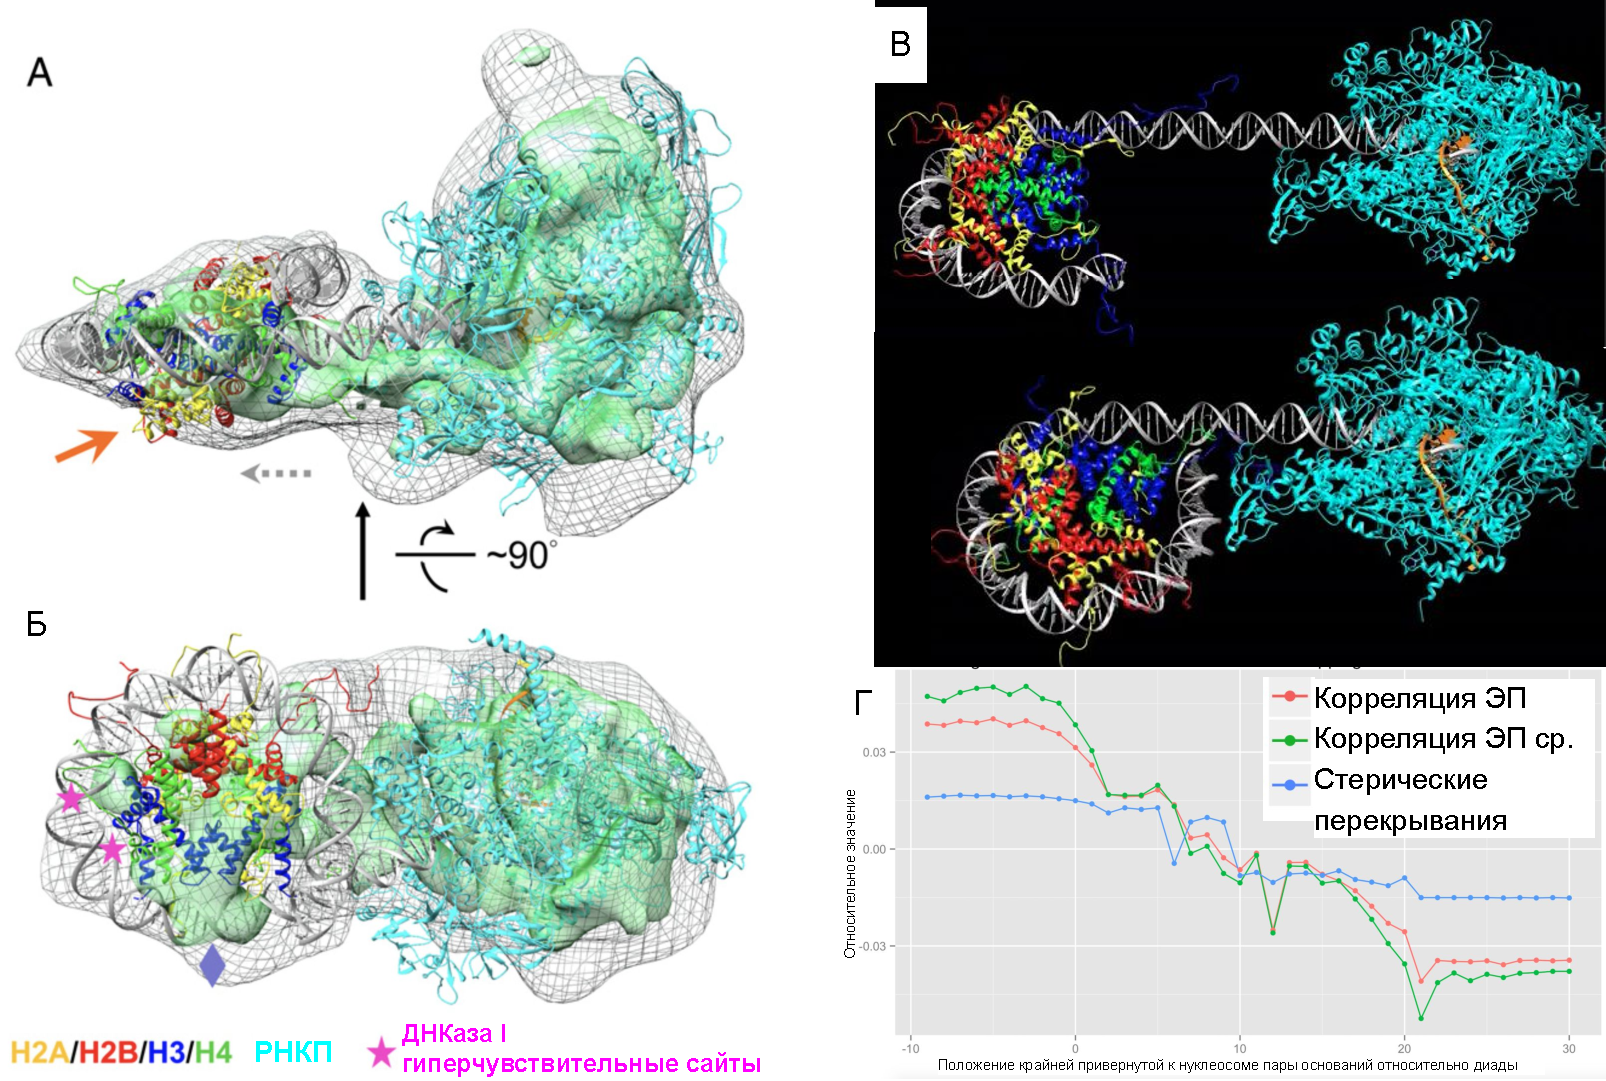
\includegraphics[width=\textwidth]{images/p6/p6_2/p6_2_pnas_f6.pdf}
    \caption[Структура комплекса элонгации остановленного в положении +42 нуклеосомы.]{Структура комплекса элонгации остановленного в положении +42 нуклеосомы. (A) Модель ЭК +42, построенная путем подбора оптимальной структуры комплекса, вписывающейся в электронную плотность, полученную экспериментально. Изоповерхность трехмерной реконструкции электронной плотности показана с более высоким или низким порогом серой сеткой или зеленым цветом, соответственно. Серая пунктирная и оранжевая стрелки указывают направление транскрипции и промотор-проксимальный димер H2A / H2B, экспонированный в раствор, соответственно. (Б) Структура была повернута на 90$^\circ$ вокруг горизонтальной оси. Положение участков ДНК, гиперчувствительных к ДНКазе I, показано звездочками. Нуклеосомная диада обозначена фиолетовым ромбом. (В) Различные варианты модели, отличиющиеся отворотом ДНК. (Г) График корелляции плотности модели и экспериментальной электронной плотности.}
    \label{fig:p6_2_pnas_f6}
\end{figure}
   
   
   Спейсер ДНК в полученной модели, соединяющий нуклеосому и РНКП, в значительной степени скрыт белками; таким образом структура согласуется с данными футпринтинга ДНКазы I, не обнаруживающими доступности спейсерной ДНК. Плотная структура комплекса согласуется с предположением, что у остановленного комлекса откат полимеразы сопровождается прикручиванием нуклеосомной ДНК к поверхности октамера гистонов. Докинг структуры элонгационного комплекса дрожжей Pol II в полученную модель свидетельствует о том, что подобный комплекс может быть образован эукариотический Pol II.
    
    Самая яркая и удивительная особенность комплекса +42 - это экспонирование поверхности промотор-проксимального димера гистонов H2A/H2B, взаимодействующего с ДНК. Действительно, модель +42 комплекса (рис. \ref{fig:p6_2_pnas_f6}) предполагает, что проксимальный участок H2A / H2B димера не стабилизируется взаимодействием с ДНК или РНКП, но остается связанным с октамером. Кроме того, наши предыдущие данные показали, что переход от комплекса +42 к +49 сопровождается полным приворотом нуклеосомной ДНК обратно на поверхность димера \cite{kulaeva_mechanism_2009}, предполагая, что димер не покидает ДНК до того, как Pol II продвинется более чем на 49 п.н. в нуклеосому. Стабильность димера во время транскрипции примечательна, учитывая, что октамер, свободный от ДНК, полностью теряет оба димера H2A / H2B менее, чем за 1 с \cite{feng_lifetime_1993}. Таким образом наличие нуклеосомной ДНК, которая остается частично накрученной вокруг тетрамера H3/H4 и промотор-дистального димера H2A/H2B приводит к снижению скорости диссоциации промотор-проксимального димера. Данные свидетельствуют о том, что связывание промотор - проксимального димера H2A/H2B с тетрамером H3/H4 в +42 комплексе может быть аллостерически стабилизировано оставшимися ДНК-гистоновыми взаимодействиями в нуклеосоме. Поскольку смещение димера представляет собой первый шаг к вытеснению всего октамера гистонов \cite{bintu_elongation_2011}, этот механизм, вероятно, важен для выживания нуклеосом во время различных процессов, включая ремоделирование нуклеосом.
    
    
    
   
    
\subsubsection{Обсуждение}
%2S дать красный текст pnas2015
    
    Наши данные идентифицируют переход из положения +48 в положение +49 как ключевой этап транскрипции через нуклеосому, где Pol II делает выбор между остановкой и дальнейшей транскрипцией. В минимальной системе, содержащей только Pol II и нуклеосому, этот выбор продиктован прежде всего последовательностью нуклеосомной ДНК, определяющей сродство ДНК-гистоновых взаимодействий и вероятность возврата Pol II. Особенно, Последовательность ДНК в области +(99–102) имеет решающее значение для выхода из положения +48.
    
    После преодоления нуклеосомного барьера в дальнейшем Pol II транскрипция обычно сопровождается выживанием нуклеосом благодаря образованию небольшой внутринуклеосомной петли ДНК на поверхности октамера гистонов. Высокая эффективность выживания нуклеосом оставалось загадкой, потому что транскрипция различными РНК-полимеразами сопровождается разворачиванием протяженного участка ДНК (до 80 п.н.) от октамера \cite{kulaeva_mechanism_2009,chang_structural_2013,bednar_nature_1999}, который, как ожидается, вызовет немедленную потерю димера H2A/H2B \cite{feng_lifetime_1993}. Наблюдаемая стабильность +42 комплекса, содержащего димер H2A / H2B, который экспонируется в растворитель свидетельствует о том, что связывание димера H2A/H2B с тетрамером H3/H4 может быть стабилизировано аллостерически и дает объяснение замечательной стабильность структуры нуклеосом во время различных процессов, включая транскрипцию \cite{kulaeva_mechanism_2009}, репликацию \cite{randall_fate_1992} и АТФ-зависимое ремоделирование хроматина \cite{mueller-planitz_nucleosome_2013}. Хотя один димер конститутивно вытесняется из нуклеосом при транскрипции \textit{in vitro} \cite{kireeva_nucleosome_2002}, это вытеснение, вероятно, происходит после транскрипции через позицию +49, поскольку ЭК+49 содержит оба димера H2A/H2B \cite{churchman_nascent_2011}.
    
    Описанная здесь паузирование в положениях +42/48 наблюдается у \textit{Drosophila} \cite{weber_nucleosomes_2014} и дрожжей \cite{churchman_nascent_2011}. В дрожжах первичный нуклеосомный барьер во время удлинения транскрипта  Pol II встречается, когда активный центр фермента находится в области +(40–55) п.н. в нуклеосоме . С аналогичным барьером сталкивается Pol II у дрозофилы во время транскрипции через нуклеосомы, локализованные на расстоянии более $\sim$400 п.н. от сайтов старта транскрипции \cite{weber_nucleosomes_2014}. Однако существуют дополнительные нуклеосомные барьеры в позициях -7 и +20 п.н. у Drosophila, характерные для нуклеосом, локализованные сразу после сайта старта транскрипции \cite{weber_nucleosomes_2014}.
    
    Недавние исследования показывают, что плотность комплексов Pol II вдоль транскрибированных генов, вероятно, определяет важные параметры транскрипции через хроматин - высоты нуклеосомных барьеров \cite{kulaeva_rna_2010,jin_synergistic_2010,chang_analysis_2014}, степень смещения гистонов и их обмен \cite{lee_evidence_2004,kulaeva_rna_2010,dion_dynamics_2007,rufiange_genome-wide_2007}. В то же время множественные факторы, включая модификации гистонов, варианты гистонов, шапероны гистонов и ремоделеры хроматина, дополнительно изменяют динамику гистонов на транскрибируемых генах \cite{smolle_resetting_2013,das_histone_2013,zentner_regulation_2013,weber_histone_2014}. Некоторые из эти факторов взаимодействуют с опухолевыми супрессорами \cite{wen_zmynd11_2014} и представляют важные мишени для разработки противоопухолевых препаратов \cite{garcia_facilitates_2013}.
    
    
    
    
    
    
    
    
    
    
    
    
    
    
    
    
    
    
    
    
    
    
    
    
    

\section{Конформационные перестройки нуклеосом при взаимодействии с комплексом FACT}
\textit{Текст данного раздела основан на статье \cite{valieva_large-scale_2016}}.
%2S -необходимо взять материал из materials/Armeev_disser.pdf пункт 4.5 (со стр 71) небходимо переформулировать так, чтобы не нашел антиплагиат
    
  
  Динамика нуклеосом может активно регулироваться взаимодействиями с различными белками. Нашими коллегами был произведен ряд экспериментов методом spFRET для изучения конформационных перестроек в нуклеосомах при его взаимодействии с комплексом шаперонов FACT. В ходе эксперимента был введен ряд пар меток (Cy3-Cy5) разные положения нуклеосомной ДНК: проксимальные метоки - вблизи входа в нуклеосому, медиальные - по центру нуклеосомы и дистальные - вблизи выхода из нуклеосомы (Рис. \ref{fig:p6_3_f22}). По изменению сигнала spFRET было обнаружено, что связывание FACT вызывает существенные, но обратимые изменения в сигнале FRET. С использованием этих данных методами интегративного моделирования нами были построены модели возможных конформационных перестроек в нуклеосомах.
    
\begin{figure} [H]
    \centering
    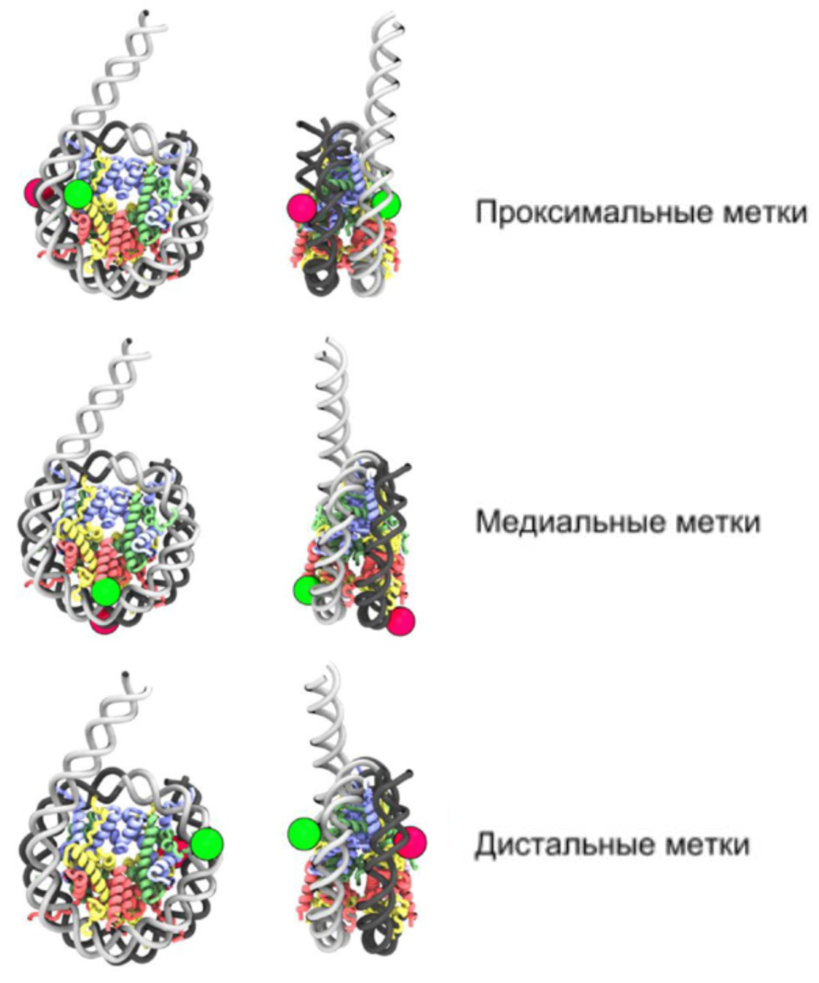
\includegraphics[width=\textwidth]{images/p6/p6_3/p6_3_f22.pdf}
    \caption[Расположение флуоресцентных меток на нуклеосоме в spFRET экспериментах]{Расположение флуоресцентных меток на нуклеосоме в spFRET экспериментах. Зеленым показаны положения донора (Cy3), красным - акцептора (Cy5).}
    \label{fig:p6_3_f22}
\end{figure}
    
    
    
    На основе измерений, в том числе с использованием измерения фактора детекции (см. главу \ref{part1_1_md}), нами был сконструирован и отобран ряд возможных моделей, которые согласуются с экспериментальными данными. Установлено, что для  значительного изменения эффективности переноса, наблюдаемого в эксперименте, величина откручивания ДНК от нуклеосомы должна составлять около 100 н.п. ДНК, при этом около 40 н.п. должно откручивать с одной стороны и около 60 н.п. с другой стороны (рис. \ref{fig:p6_3_f23}).
    
\begin{figure} [H]
    \centering
    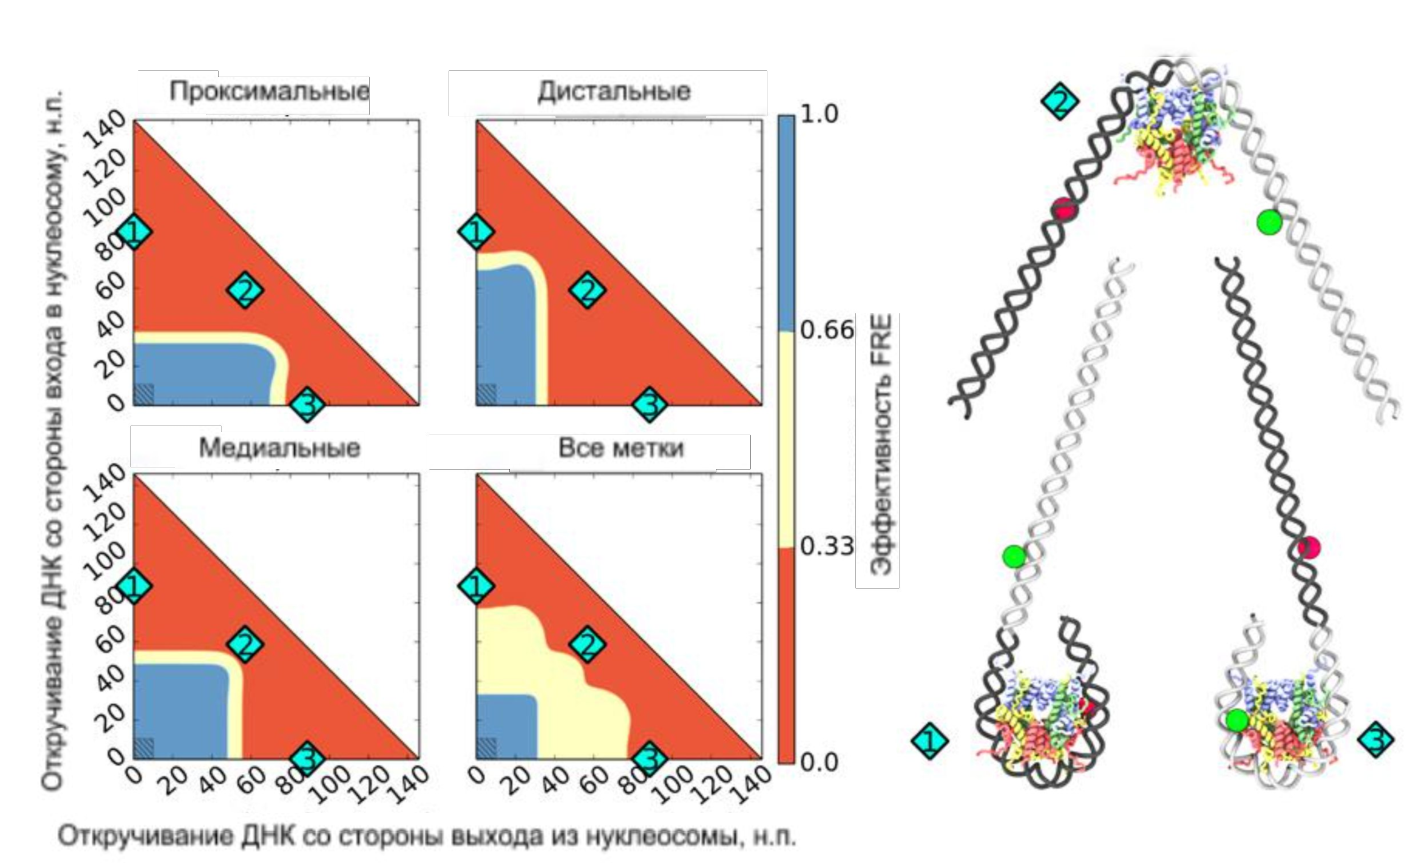
\includegraphics[width=\textwidth]{images/p6/p6_3/p6_3_f23.pdf}
    \caption[Анализ зависимости эффективности FRET от степени разворачивания нуклеосом]{Анализ зависимости эффективности FRET от степени разворачивания нуклеосом. Слева: тепловые карты ожидаемых эффективностей переноса энергии на трех парах флуорофоров. Красные и голубые области соответствуют степеням откручивания ДНК с низкой и высокой эффективностью FRET соответственно. Затемненные участки тепловых карт (левый нижний угол) отвечают нативным состояниям нуклеосом (состояниям близким к наблюдаемым в кристаллических структурах). Справа: Модели конформаций нуклеосом, соответствующие отмеченным номерам на картах.}
    \label{fig:p6_3_f23}
\end{figure}
    
    По этим данным были построены молекулярные модели, соответствующие таким степеням отворота ДНК (Рис. \ref{fig:p6_3_f24}): модель откручивания ДНК с сохранением гистонового октамера (Рис. \ref{fig:p6_3_f24}), модель откручивания ДНК с образованием структуры ``бабочка'' (Рис. \ref{fig:p6_3_f24}3) , модель с образованием двух хемисом (Рис. \ref{fig:p6_3_f24}5), а также модель полного разрушения октамера гистонов (Рис. \ref{fig:p6_3_f24}). Все эти модели в равной степени соответствуют наблюдаемым изменениям в эффективности переноса энергии в присутствии гистонового шаперона FACT.
    
\begin{figure} [H]
    \centering
    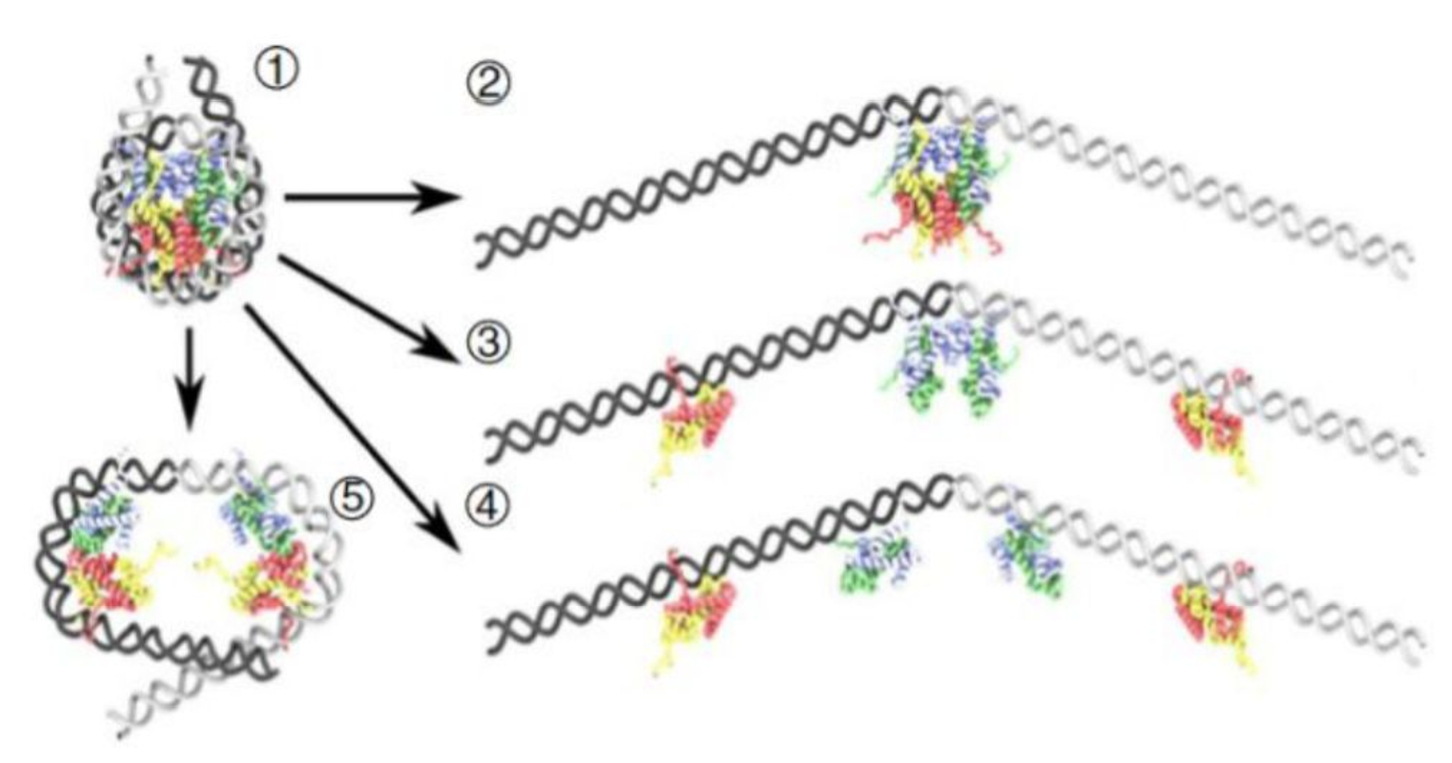
\includegraphics[width=\textwidth]{images/p6/p6_3/p6_3_f24.pdf}
    \caption[Модели разворачивания нуклеосом, вызванного взаимодействием с шапероном FACT]{Модели разворачивания нуклеосом, вызванного взаимодействием с шапероном FACT. Интактные нуклеосомы (1) могут разворачиваться от интактного октамера (2), ДНК может отворачиваться с разрушением (3) или без (4) разрушения интерфейса взаимодействия гистонов H3–H3 или путем открытия интерфейса H3-H3 без откручивания ДНК (5) с формированием двух хемисом.}
    \label{fig:p6_3_f24}
\end{figure}
    
    Потеря гистонов в процессе откручивания ДНК при низких концентрациях нуклеосом должна быть необратимой, так как в ходе экспериментов в раствор дополнительно добавляли конкурирующую за гистоны ДНК, не меченную флуорофорами. Тот факт, что наблюдаемый эффект был обратим, свидетельствует о том, что разворачивание октамера должно происходить без потери гистонов H2A-H2B.
    
    
    
    
    
    
    
    
    
    
    
    
    
    
    
    
    
    
    
    
    
    
    
    
    
    
    
    
    
    
    
    
    
    
    
    
    
    
    
    
    
    
    
    
    
    
    
    
    
    
    
    
    
    
    
    
    
    
    
    
    
    

\section{Модели взаимодействия нуклеосом с белком CENP-C}
\textit{Текст данного раздела основан на статье \cite{xiao_molecular_2017}}.
%2S необходимо литературу проставить, оригинальная статья тут materials/gesdev2017/genesdev2017.pdf
%2S нужно перевести вот эту картинку https://docs.google.com/drawings/d/1Wa7FAkYUa-TmG-6vC0wwXJO0_HeVc04UCN8hmnvNM7I/edit

\subsection{Введение}
Кинетохоры представляют собой большие субклеточные структуры из $\sim$75 полипептидов, которые собираются на центромерах хромосом, чтобы сделать возможным точное разделение реплицированных дочерних хромосом во время деления клеток \cite{fukagawa_centromere_2004,biggins_composition_2013}. Открытие трех центромер-специфичных аутоантигенов человека, обозначенных CENP-A (гистоновый вариант CenH3), CENP-B (специфичный для последовательности фактор связывания ДНК спираль-виток-спираль) и CENP-C (компонент внутреннего кинетохора), проложили путь к пониманию центромерного хроматина на молекулярном уровне и его роли в сборке кинетохор \cite{fukagawa_centromere_2014}. На фундаментальном уровне нуклеосомы замена канонического гистона H3 на CENP-A в специфичных для центромеры нуклеосомах создает платформу для рекрутирования CENP-C \cite{carroll_dual_2010,gascoigne_induced_2011}. CENP-C колокализуется с CENP-A на центромерах многоклеточных животных и служит структурной связи между нуклеосомами CENP-A и белками внешней кинетохоры, тем самым соединяя центромеры с микротрубочками для сегрегации хромосом \cite{moroi_autoantibody_1980,earnshaw_identification_1985,saitoh_cenp-c_1992,sullivan_determining_2001,biggins_composition_2013}. CENP-C является ключевым компонентом мультисубъединичного комплекса CCAN (конститутивной сеть, ассоциированная с центромерой), образующего внутреннюю часть кинетохоры \cite{weir_insights_2016}. Следовательно, молекулярные основы взаимного узнавания между CENP-C и нуклеосомой CENP-A является центральным фактором для понимания того, как внутренняя кинетохора взаимодействует с центромерным хроматином.

Центральная часть полипептида CENP-C содержит три консервативных домена, важных для узнавания центромеры: высококонсервативный ``сигнатурный мотив CENP-C'', который контактирует с гидрофобным C-концом CENP-A \cite{carroll_dual_2010,kato_conserved_2013}, центральная ДНК-связывающая область, которая содержит CENP-C-подобный мотив, и домен гомодимеризации \cite{brown_sequence_1995,yang_identification_1996,sugimoto_characterization_1997,politi_cenp-c_2002,milks_dissection_2009,trazzi_c-terminal_2009}. У почкующихся дрожжей, гомолог CENP-C Mif2 \cite{meeks-wagner_isolation_1986} не обладает специфической для позвоночных ДНК-связывающей областью, но он содержит один мотив CENP-C и один ``AT-крюк'' \cite{brown_sequence_1995,huth_solution_1997,reeves_structure_2000}. Ранние исследования показали, что AT-крюк в Mif2 способствует узанванию центромер и сегрегации хромосом \textit{in vivo} \cite{brown_sequence_1995,lanini_domains_1995,meluh_evidence_1995,cohen_structural_2008}. Более того, N-концевой домен в Mif2 ассоциируется с двумя кинетохорными белками (Ame1-Okp1), чтобы облегчить сборку внешних кинетохор \cite{hornung_cooperative_2014}.

\subsection{Построение модель взаимодействия на основе данных футпринтинга ДНК}
Для понимания взаимодействия Mif2 с центромерными нуклеосомами \textit{in vitro} была проведена серия экспериментов по футпринтингу комплексов гидроксильными радикалами. Для обработки и интерпретации данных была применена программа HYDROID описанная в главе \ref{part5_hrf}, а также построенная нами и описанная в той же главе модель центромерной нуклеосомы.

ДНК центромеры дрожжей длиной 125 п.н. состоит из трех смежных генетических элементов: CDEI, CDEII и CDEIII \cite{hegemann_centromere_1993}. Мы использовали метод футпринтинга ДНКазой I для определения сайта связывания димера Mif2c на нуклеосоме Cse4/CEN3 -- участка длиной  $\sim$30 п.н. в пределах AT-богатого элемента CDEII ($\sim$85 п.н.) на одной стороне от диады нуклеосомы в направлении CDEIII. Для дальнейшего картирования точных контактов Mif2-ДНК мы выполнили футпринтинг димера Mif2c на нуклеосоме Cse4/CEN3 методом гидроксильного футпринтинга. Поскольку гидроксильный радикал представляет собой небольшую молекулу, от его атаки защищены только места тесных контактов. Как показано на рисунке  \ref{fig:p6_5_f5}, димер Mif2c защищает $\sim$30 п.н. ДНК от расщепления гидроксильным радикалом, что в высокой степени согласуется с защитой от ДНКазы I. Учитывая, что минимальный сайт для связывания  Mif2 лишенного димеризационного домена составляет 16-18 п.н., защита в 30 п.н. при связывании димера Mif2c предполагает, что оба ДНК-связывающих домена из димерного Mif2 взаимодействует с одной стороной нуклеосомы.

Это поднимает вопрос, почему димер Mif2 должен связываться только с одной стороной нуклеосомы, когда обе стороны состоят примерно из эквивалентного процента AT. Мы исследовали эту проблему и обнаружили второй, более медленный по подвижности в геле комплекс при двукратном или трехкратном увеличении концентрации димера Mif2c в реакции связывания. Анализ гидроксильным футпринтингом показывает, что обе стороны нуклеосомной диады этого комплекса теперь защищены от расщепления гидроксильными радикалами (данные не показаны). Таким образом, одна нуклеосома Cse4 / CEN3 способна связываться с двумя димерами Mif2, занимающими каждую сторону нуклеосомы. Связывание с AT-богатой ДНК является доминирующим фактором, но правила предпочтительного связывания со специфической AT-богатой последовательностью остаются неясными. Мы предполагаем, что точное расположение пары оснований AT может придавать тонкие различия в гибкости и / или конформации ДНК, делая одну AT-богатую сторону от диады более привлекательной, чем другую.

Чтобы определить, является ли сайт между диадой нуклеосомы и CDEIII  предпочтительным для взаимодействий Mif2 на других центромерных нуклеосомах, мы выполнили эксперименты по футпринтингу нуклеосом, реконструированных на CEN10. Интересно, что сайт связывания димера Mif2c был картирован в AT-богатых регионах на противоположной стороне от нуклеосомной диады для CEN10, по направлению к CDEI. Таким образом, Mif2 взаимодействует с нуклеосомой Cse4 в соседнем с диадой сайте внутри CDEII, но его ориентация связывания относительно оси диады, по-видимому, специфична для каждой конкретной центромеры. Это означает, что определенные паттерны последовательности лежащей в основе AT-богатой ДНК предпочтительнее для Mif2. Чтобы проверить, отражают ли  области повышенной защиты, наблюдаемые в нуклеосомах при связывание димера Mif2c, какие-либо свойства ДНК самой по себе, мы выполнили реакции футпринтинга ДНКазы I с голой ДНК CEN3. Мы не наблюдали никаких специфических следов связывания для димера Mif2c на голой ДНК CEN3. Это указывает на то, что сайт-специфическая локализация Mif2 на нуклеосоме требует вовлечения как ДНК, так и гистоновых сигналов Cse4.

\begin{figure}[H]
    \centering
    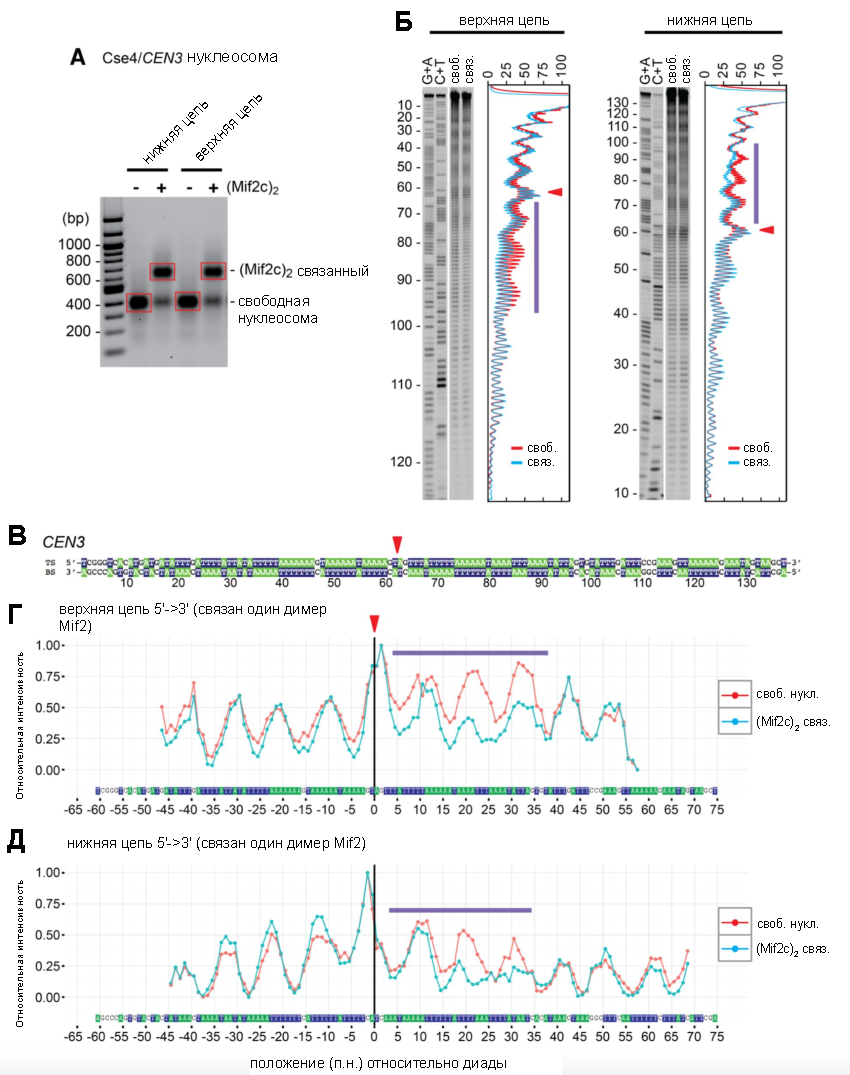
\includegraphics[width=0.9\textwidth]{images/p6/p6_4/p6_5_f5.pdf}
    \caption[Анализ комплексов димеров Mif2 с центромерными нуклеосомами Cse4/CEN3 методами гидроксильного футпринтинга]{Анализ комплексов димеров Mif2 с центромерными нуклеосомами Cse4/CEN3 методами гидроксильного футпринтинга. (A) Анализ комплексов с помощью агарозного гель электрофореза после расщепления ДНК гидроксильными радикалами. (Б) Изображения продуктов реакции после ПААГЭ. Красные линии  - нуклеосомы, голубые - нуклеосомы с димером Mif2c. (В) Положение  диады на ДНК для Cse4/CEN3 нуклеосомы (см. главу \ref{part5_hrf}). (Г, Д) Профили интенсивности расщепления гидроксильными радикалами цепей ДНК в нуклосомах с и без Mif2. Фиолетовые линии - дополнительная защита от расщепления.}
    \label{fig:p6_5_f5}
\end{figure}

\subsection{Обсуждение}
Понимание работы центромер многоклеточных животных представляют собой некоторый парадокс, потому что их последовательности сильно расходятся даже между родственными видами, несмотря на функциональную законсервированность \cite{henikoff_centromere_2001}. Неуловимая природа универсального паттерна последовательности повторяющихся ДНК активных центромер многоклеточных животных привела к широкому признанию того, что идентичность центромер управляется эпигенетическими механизмами; т.е. за счет сборки и свойств унаследованного гистона CENP-A, а не лежащей в основе последовательности ДНК центромеры \cite{sullivan_determining_2001,allshire_epigenetic_2008,black_epigenetic_2011}. Заметным исключением является строго генетически определенная позиция центромер почкующихся дрожжей, где нуклеосомный гистон Cse4/CENP-A деградирует при переходе G1 – S каждого клеточного цикла, что исключает эпигенетическую передачу \cite{biggins_composition_2013,wisniewski_imaging_2014}. Вместо этого центромерный хроматин восстанавливается \textit{de novo} с помощью инструкций от трех специфических элементов последовательности (120 п.н.) центромеры дрожжей и их множественных родственных факторов \cite{westermann_structures_2007}. Интересно, что ранее существовавший Mif2 на центромере почкующихся дрожжей передается дочерним клеткам; значение этой передачи еще предстоит изучить.

В этой работе мы выделили отличительные особенности AT-богатой центромеры дрожжей ДНК. Варианты как ДНК, так и гистонов вносят вклад в тысячукратное усиление связыания Mif2 с центромерными нуклеосомами по сравнению с перицентромерным. Это огромное предпочтение, вероятно, лежит в основе сайт-специфичности нуклеации кинетохор, хотя другие механизмы могут вносить свой вклад; напр. взаимодействия с участием N-концевого хвоста Cse4 \cite{chen_n_2000,samel_methylation_2012} и взаимодействия между N концом Mif2 и кинетохорными компонентами CENP-UAme1-CENP-QOkp1 \cite{hornung_cooperative_2014}. Дальнейший вклад в селективность нуклеосом CENP-A по сравнению с нуклеосомами H3 может также происходить от компонентов CCAN \cite{weir_insights_2016}.

Мы подтвердили важность Cse4-гидрофобного С-конца для взаимодействий Mif2, что согласуется с предыдущими исследованиями \cite{carroll_dual_2010,guse_vitro_2011,kato_conserved_2013}. Однако, хотя вклад гистоновых фолдов CENP-A ранее был исключен \cite{guse_vitro_2011}, мы обнаружили явную важность петли L1, несущей три дополнительных заряженных и полярных остатка (KDQ), и спирали $\alpha$-2 Cse4. Однако, как мы показали весьма важной является и вклад последовательности ДНК в связывание Mif2. Какие особенности  AT-богатой CDEII последовательности длиной 85-п.н. способствуют связыванию Mif2? Область защиты ДНК от расщепления гидроксильными радикалами длиной $\sim$30 п.н., возникающая в результате связывания димера Mif2, покрывает большую часть одной AT-богатой стороны нуклеосомы. CDEII для всех 16 центромер дрожжей содержат несколько коротких участков An$\cdot$Tn или Tn$\cdot$An трактов плюс динуклеотидные шаги ApT или TpA между участками. Длина и расположение трактов различаются между центромерами \cite{baker_genetic_2005}. Тракты An$\cdot$Tn и Tn$\cdot$An обладают узкой малой бороздкой, большим пропеллерным разворот оснований (propeller twist), а также бифуркационными водородными связями, которые улучшают стэкинг оснований и жесткость спирали \cite{coll_bifurcated_1987,nelson_structure_1987}. С другой стороны, шаги динуклеотидов TpA (но не шаги ApT) обнаруживают расширенные малые бороздки на стыках трактов \cite{stefl_dna_2004}. Одна из этих или обе геометрические особенности AT-богатой ДНК могут изменять обычные спиральные параметры нуклеосомной ДНК, намотанной на гистоновое ядро (Bishop et al. 2011). Например, кристаллическая структура одного длинного тракта A16$\cdot$ T16 на канонической нуклеосоме выявила локальное искажение спирали нуклеосомной ДНК \cite{bao_nucleosome_2006}.

Учитывая корреляцию между предпочтением связывания Mif2 и AT-богатым составом ДНК, мы предполагаем, что конформации AT-богатого CDEII распознаются AT-крюк и кластерами аминокилот аргинина и лизина (RK) Mif2. Mif2 имеет один классический AT-крюк (GRPRGRPK) на С-конце своего ДНК/гистон связывающего домена. Структурные исследования показали, как отдельные остатки AT-крюков взаимодействуют с узкими малыми бороздками родственных AAAT и AATT элементов \cite{reeves_t-dna-binding_1990,huth_solution_1997,reeves_structure_2000}. Аргинины и, в меньшей степени, лизины кластеров RK широко используются для во взаимодействии белок-ДНК не только гистонового ядра нуклеосомы \cite{luger_crystal_1997}, но также и факторов транскрипции, специфичных для последовательности животных, таких как как UBX, OCT1, бактериальный репрессор MogR \cite{rohs_role_2009,rohs_origins_2010,shen_recognition_2009,kong_functional_2015}. Мы предполагаем, что кластеры RK, используют этот способ взаимодействия с ДНК как часть своей стратегии по специфическому связыванию. Мы предполагаем, что наши результаты закладывают важные основы для дальнейших исследований и уточнению структурно-динамической модели взаимодействия Mif2 с центромерными нуклеосомами.

\section{Анализ комплексов нуклеосомы и гистона H1}
\textit{Текст данного раздела основан на статьях \cite{gorkovets_joint_2018,armeev_modeling_2016} }.

%2S тут нужно проставить литературу - список литературы дан после каждой подсекции
\subsection{Совместное влияние аминокислотной последовательности гистона H1 и нуклеотидной последовательности ДНК на структуру хроматосомы: анализ методами молекулярного моделирования}

\textit{Текст ниже приведен согласно статье \cite{gorkovets_joint_2018} <<}

Хроматосома, состоящая из нуклеосомного ядра, линкерных участков ДНК и линкерного гистона H1 (ЛГ), является важным структурным элементом хроматина. Существует два экспериментально подтвержденных типа связывания ЛГ с нуклеосомой и линкерной ДНК, которые различаются своей геометрией - связывание ``на диаде'' и ``вне диады''. Показано, что на тип связывания гистона и конформацию хроматосомы влияет аминокислотная последовательность ЛГ.  Однако, при связывании ЛГ изменяется в том числе и геометрия линкерной ДНК. Взаимовлияние этих факторов и молекулярные основы, определяющие тип связывания ЛГ и нуклеосомы, остаются неясными. В данной работе мы применили методы молекулярного моделирования, включая моделирование по гомологии, анализ атом-атомных взаимодействий и расчет энергии деформации ДНК для изучения совместного влияния аминокислотной последовательности ЛГ и нуклеотидной последовательности ДНК на конфигурацию хроматосомы. Были проанализированы известные кристаллические и ЯМР структуры хроматосомы на предмет атом-атомных взаимодействий ЛГ и ДНК, а также энергии деформации ДНК в этих структурах для различных последовательностей ДНК. Для различных вариантов ЛГ анализ проводился с использованием методов моделирования по гомологии. Были обнаружены зависящие от последовательности различия в энергии изгиба линкерной ДНК для двух различных конформаций хроматосомы, а также предложены нуклеотидные последовательности, предпочтительные для этих структур. В результате анализа было показано, что нуклеотидная  последовательность ДНК наряду с аминокислотной последовательностью ЛГ оказывает влияние на тип связывания с нуклеосомой. Сформулированы гипотезы для экспериментальной проверки, согласно которым тип связывания ЛГ может меняться при изменении нуклеотидной последовательности ДНК. 

Структурными единицами хроматина являются нуклеосомы - ДНК-белковые комплексы, содержащие гистоны. Ядро нуклеосомы образовано октамером гистонов H2A, H2B, H3 и Н4, вокруг которого располагается двойная спираль ДНК длиной около 146 пар оснований \cite{luger_crystal_1997}. Нуклеосома обладает осью псевдосимметрии второго порядка, называемой также диадной осью (рисунок \ref{fig:p6_5_f1}А). Эта ось проходит через центр нуклеосомальной ДНК, называемый диадой.
Следующим уровнем компактизации является хроматосома \cite{simpson_structure_1978}, образованная при связывании линкерного гистона H1 (ЛГ) и нуклеосомы, включающей линкерные участки ДНК, выходящие за пределы ядра нуклеосомы (рисунок \ref{fig:p6_5_f1}А). Таким образом, в хроматосому входит октамер гистонов H2A, H2B, H3 и Н4, нуклеосомальная ДНК, ЛГ  и линкерные участки ДНК. 
ЛГ представлены во многих эукариотических организмах несколькими вариантами, различающимися длиной аминокислотной последовательности и ее составом \cite{lyubitelev_structure_2016}. В различных клетках и тканях могут экспрессироваться различные варианты ЛГ. Как правило, у наиболее просто устроенных организмов встречается всего один вариант ЛГ, тогда как, например, у человека известно 11 вариантов \cite{el_kennani_ms_histonedb_2017}, некоторые из которых экспрессируются только в половых клетках. Также стоит отметить, что присутствие того или иного варианта ЛГ зависит не только от типа клетки, но и от стадии клеточного цикла, в которой она находится.
Большая часть ЛГ содержит около 200 аминокислотных остатков. ЛГ состоят из трех доменов: короткий и неупорядоченный N-конец, за которым идет глобулярный домен, образованный 70-80 аминокислотными остатками и имеющий консервативную третичную структуру, и длинный С-концевой домен из примерно 100 аминокислотных остатков. С-конец является неорганизованным и содержит много остатков лизина. Согласно экспериментальным данным \cite{syed_single-base_2010} глобулярный домен ЛГ связывается с нуклеосомой наравне с полноразмерным ЛГ. Ввиду большой степени неупорядоченности концевых доменов отсутствуют кристаллические структуры полноразмерного ЛГ, но существуют кристаллические структуры глобулярного домена \cite{ramakrishnan_crystal_1993}.
В данный момент областью для обсуждений является конфигурация связывания ЛГ с нуклеосомой. Ранее существовали различные модели связывания ЛГ с нуклеосомой. Некоторые из них даже предполагали встраивание ЛГ между витками нуклеосомальной ДНК и октамером гистонов \cite{pruss_asymmetric_1996}. Подобные модели не нашли впоследствии экспериментального подтверждения \cite{syed_single-base_2010,zhou_position_1998} в отличие от моделей, в которых предполагается связывание ЛГ в области диады нуклеосомы и линкерных участков ДНК. 
Имеющиеся на текущий момент экспериментальные данные \cite{bednar_structure_2017,zhou_structural_2013,zhou_structural_2015,zhou_small_2016} предполагают два возможных расположения ЛГ в хроматосоме, условно называемые как «на диаде» (НД, ``on-dyad'') и «вне диады» (ВД, ``off-dyad''). На данный момент получена кристаллическая структуры хроматосомы с глобулярным доменом ЛГ H5 \textit{G. gallus} (H5 является историческим названием ЛГ Н1 у \textit{G. gallus}) в конфигурации НД, а также модель структуры хроматосомы с глобулярным доменом ЛГ Н1 \textit{D. melanogaster} в конфигурации ВД \cite{zhou_structural_2015}. Важно отметить, что структура хроматосомы в конфигурации ВД была построена с помощью методов молекулярного докинга на основании структуры тетрануклеосомы (pdb-код 1zbb) на основании данных ЯМР. 
Известно, что ЛГ содержит ряд аминокислотных остатков, играющих важную роль в формировании контактов с нуклеосомой \cite{brown_mapping_2006}. Эти остатки выделены в два сайта связывания: первый - H25, R47, K69, K73, R74, K85, и второй - R42, R94, K97.
Глобулярный домен гистона Н5 \textit{G. gallus} продемонстрировал связывания типа НД с нуклеосомой, тогда как глобулярный домен Н1 \textit{D. melanogaster} продемонстрировал связывание типа ВД. Анализ их последовательностей показал отличия, вероятно играющие роль в предпочтительности того или иного типа связывания. Так, глобулярный домен Н5 содержит положительно заряженные аминокислотные остатки (R47, K55, R74, K97) в позициях соответствуюих нейтрально заряженным аминокислотным остаткам в глобулярном домене Н1 (L68, T76, S96, A119), и нейтрально заряженные аминокислотные остатки (Q51, V80, V87) в позициях соответствующим положительно заряженным остатками Н1 (K72, K102, K109) \cite{zhou_structural_2015,zhou_small_2016}. Несмотря на то, что некоторые из ключевых остатков не образуют прямых контактов с нуклеосомой, при их замене в глобулярном домене Н5 на аминокислотные остатки, характерные для Н1, ЛГ показал изменение типа связывания с НД на ВД \cite{zhou_small_2016}.
Другим фактором, который предположительно может оказывать влияние на конфигурацию хроматосомы, является нуклеотидная последовательность ДНК, как линкерной, так и входящей в состав нуклеосомы. По данным исследования позиционирования нуклеосом выдвигались предположения, что ЛГ предпочтительно связывается с АТ-богатыми участками ДНК \cite{cui_distinctive_2009}. 
Несмотря на то, что в полученной кристаллической структуре хроматосомы ЛГ показал связывания НД, по данным, полученным методами молекулярного моделирования \cite{ozturk_conformational_2016,pachov_structure_2011}, глобулярный домен ЛГ Н5 может также демонстрировать тип связывания ВД. Одним из объяснений может служить тот факт, что нуклеотидные последовательности ДНК, используемые при моделировании, отличались от нуклеотидной последовательности, для которой была разрешена кристаллическая структура НД конформации комплекса нуклеосомы с глобулярным доменом Н5 \cite{zhou_structural_2015}.
В описанных выше работах рассматривается связывание ЛГ с одиночной нуклеосомой in vitro, тогда как в клетке представлены структуры более высокого уровня компактизации - 30 нм фибриллы, представляющей собой цепочку из нуклеосом и ЛГ, связанных с линкерной ДНК. Согласно последним данным крио-электронной микроскопии в структуре 30 нм фибриллы, образованной 12 нуклеосомами, ЛГ демонстрирует связывание ВД, что может быть обусловлено геометрией линкерной ДНК в структуре фибриллы \cite{bednar_structure_2017,song_cryo-em_2014}. Таким образом нельзя исключать влияние ДНК, вызванное ``узнаванием'' ЛГ специфической формы ДНК при связывании \cite{rohs_origins_2010}. 
Исходя из вышесказанного, весьма вероятно, что на тип связывания ЛГ с нуклеосомой и линкерной ДНК влияет не только аминокислотная последовательность самого гистона, но и нуклеотидная последовательность ДНК, а также структура хроматиновой фибриллы. Известно также, что при образовании комплекса белок-ДНК на силу и тип связывания оказывают влияние как прямые взаимодействия белка с парами оснований и сахаро-фосфатным остовом, так и геометрия ДНК за счет энергии ее деформации \cite{rohs_origins_2010}. Однако, несмотря на наличие структур хроматосомы в различных конфигурациях совместное влияние этих факторов ранее не изучалось.
В данной работе методами молекулярного моделирования, а именно анализа атом-атомных взаимодействий, моделирования по гомологии и оценки энергии деформации ДНК, было проведено изучение совместного влияния аминокислотной последовательности ЛГ и нуклеотидной последовательности ДНК на тип конфигурации хроматосомы. Проведенный анализ позволил предсказать наиболее предпочтительные для того или иного типа связывания нуклеотидные последовательности линкерной ДНК и сформулировать гипотезы для экспериментальной проверки.
\subsubsection{Материалы и методы}
\emph{Анализ аминокислотных последовательностей различных гистоновых вариантов}
В работе были использованы аминокислотные последовательности ЛГ, размещенные в базе данных HistoneDB \cite{draizen_histonedb_2016}. Выравнивание доступных аминокислотных последовательностей проводилось программой Muscle \cite{edgar_muscle_2004}. Для дальнейшего анализа последовательностей использовался biopython.
\emph{Моделирование по гомологии}
Моделирование по гомологии осуществлялось в программе MODELLER \cite{webb_comparative_2016,marti-renom_comparative_2000}. В качестве белков-шаблонов использовались кристаллическая структура хроматосомы в конфигурации НД с pdb-кодом 4qlc и модель хроматосомы в конфигурации ВД, полученная на основании данных ЯМР\cite{zhou_structural_2015}. Для каждого исследуемого гистона с помощью моделирования по гомологии было построено по 10 моделей, из которых на основании DOPEscore были отобраны наилучшие структуры для анализа контактов. Анализ контактов проводился с помощью программного пакета Chimera \cite{pettersen_ucsf_2004}.
\emph{Расчет энергии деформации ДНК}
Расчет зависимости деформационной энергии линкерных участков ДНК от ее последовательности производили в пространстве обобщенных переменных Tilt, Roll, Twist, Shift, Slide, Rise; переход от атомных координат к обобщенным осуществляли при помощи программы 3DNA \cite{lu_3dna_2003}. Вычисление деформационной энергии участков ДНК производили в соответствии с формулой (\ref{DNA_ener}). Для расчетов применяли набор упругих коэффициентов и средних значений для нуклеотидных пар описанный в работе \cite{olson_dna_1998}.  
Деформационную энергию определяли для всех возможных последовательностей ДНК для четырех участков ДНК (по два на каждую модель связывания ЛГ) длиной по 12 н.п. каждый. Участок ДНК, рядом с которым располагается линкерный гистон в модели ВД был назван входом в последовательность, позиционирующую нуклеосомы (ППН), противоположный участок был назван выходом из ППН. Для каждого варианта последовательности была рассчитана разница в деформационной энергии ДНК между моделями НД и ВД. Полученное распределение разниц энергий визуализировали при помощи графического представления консервативности нуклеотидов - логотипа последовательности (sequence logo) для 5% структур с наиболее положительной разницей энергий (предпочтительные для модели НД) и 5% структур с наиболее отрицательной разницей энергий (предпочтительные для модели ВД).
\subsubsection{Результаты и обсуждение}
Настоящее исследование состояло из нескольких взаимодополняющих компонент. На основе анализа экспериментальных данных были выделены ключевые остатки ЛГ, способствующие тому или иному типу связывания, на основании которых была построена классификационная модель, которая была применена к ЛГ человека: H1.1, H1.2, H1.3, H1.4, H1.5, H1.0 (H1$^\circ$), TS H1.6 (H1T), TS H1.7 (H1T2, HANP1), OO H1.8 (H1oo), TS H1.9 (HILS1), H1.10, H1.11, а также к ЛГ \textit{X. laevis}. Для экспериментально определенных структур хроматосомы и структур с различными вариантами ЛГ, построенных с помощью моделирования по гомологии были проанализированы контакты между ЛГ и ДНК. Был проведен оригинальный анализ конформации ДНК в различных структурах хроматосомы и анализ пространства последовательностей линкерных ДНК с точки зрения энергии их изгиба и контактов с ЛГ. 

\emph{Определение ключевых остатков ЛГ, влияющих на тип связывания}
Аминокислотная последовательность ЛГ имеет ряд ключевых позиций, мутации в которых приводят к изменению типа связывания \cite{zhou_small_2016}. Таким образом, на основании аминокислотных остатков, расположенных в этих позициях, для ЛГ может быть определен предполагаемый тип связывания, что позволяет предложить классификацию ЛГ по типу их связывания с нуклеосомой на основании аминокислотных последовательностей. 
В экспериментально определенной структуре хроматосомы в конфигурации НД и ВД присутствуют контакты непосредственно с парами оснований и линкерной ДНК, и нуклеосомальной ДНК, данные взаимодействия представлены как водородными связями, так и Ван-дер-Ваальсовыми взаимодействиями. 
Некоторые из аминокислотных остатков, расположенных в ключевых позициях (например, аминокислотные остатки, соответствующие K55, Q51, V87 ЛГ Н5) не образуют прямых контактов с ДНК в известных структурах. Однако, несмотря на отсутствие контактов с ДНК, данные остатки предположительно могут взаимодействовать с ДНК посредством электростатического потенциала, поскольку в гистонах Н1 и Н5 они имеют различные заряды.
\emph{Классификация ЛГ на основании наличия ключевых остатков}
На основании предложенной выше классификации, было показано, что для 3 ЛГ человека предполагаемый тип связывания был определен как НД, для 7 гистонов человека тип связывания не может быть определен однозначно, поскольку они демонстрируют сходство в ключевых позициях и с гистоном Н5 \textit{G. gallus} (тип связывания НД), и с гистоном Н1 \textit{D. melanogaster} (тип связывания ВД), для 1 гистона человека предполагаемый тип связывания может быть определен однозначно как ВД. Для ЛГ \textit{X. laevis} тип связывания был определен как НД. 

   \begin{figure} [H]
    \centering
    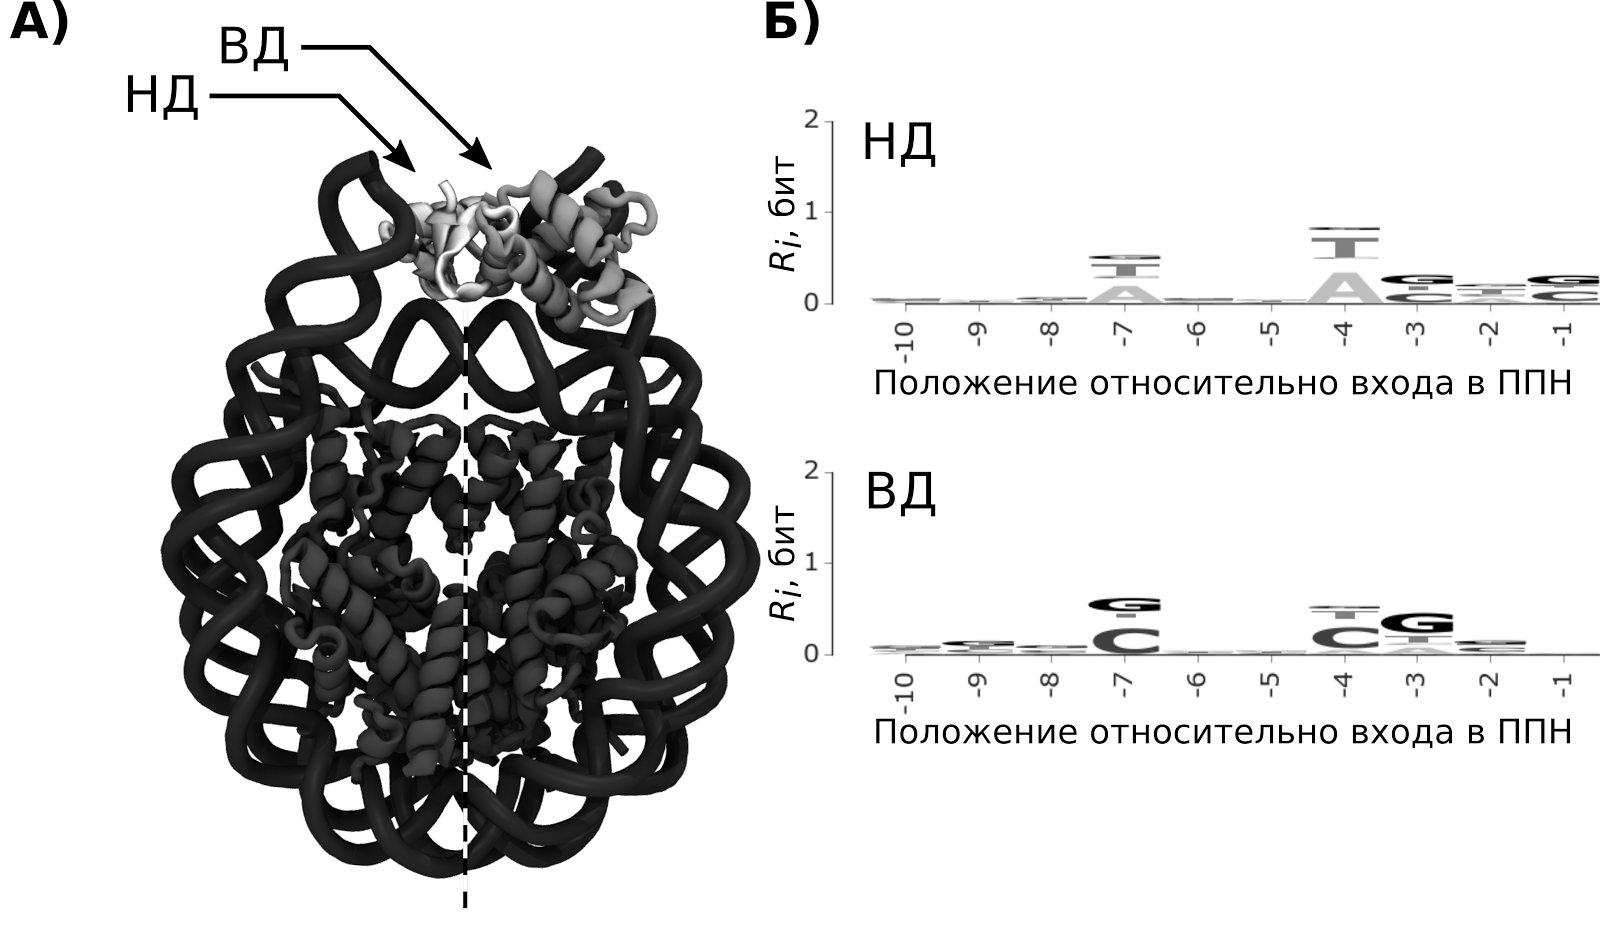
\includegraphics[width=\textwidth]{images/p6/p6_5/p6_5_f1.png}
    \caption[Cтруктура хроматосомы и оптимальные последовательности линкерной ДНК.]{Cтруктура хроматосомы и оптимальные последовательности линкерной ДНК. A) Внешний вид структуры хроматосомы. Белок и ДНК показаны в виде отображения вторичной структуры. Линкерные гистоны выделены оттенками серого. Диадная ось показана пунктирной линией.
Б) Визуализация частоты встречаемости нуклеотидов для последовательностей, склонных к формированию структуры НД (сверху) и ВД (снизу). Визуализация выполнена в виде логотипов последовательностей.
}
    \label{fig:p6_5_f1}
\end{figure}

\emph{Энергия деформации ДНК в различных конфигурациях хроматосомы}
Для определения зависимости типа связывания ЛГ от нуклеотидной последовательности линкерной ДНК была рассчитана разница деформационных энергий линкерных участков ДНК между моделями НД и ВД для всех возможных вариантов последовательностей. Также была произведена Z-оценка положения последовательности из оригинальных моделей в распределении рассчитанных деформационных энергий (Z=0,75), исходя из которой оригинальная последовательность, использованная для экспериментального получения структур, склонна к формированию структуры НД.
Как видно из рисунка \ref{fig:p6_5_f1}Б, большинство позиций в последовательностях нуклеотидов линкерных участков ДНК не значимы для определения геометрии ДНК в рамках моделей НД и ВД, кроме нуклеотидов в позициях -7, -4 и -3. В последовательностях, предпочтительных для модели НД, в этих позициях располагаются A/T, A/T, G/C, в то время как для модели ВД более предпочтительны  C/G, C/T, G/T. Богатость линкерной ДНК тимидинами также была показана в работе \cite{cui_distinctive_2009}.
Также по разнице в деформационных энергиях были найдены предпочтительные (оптимальные) последовательности линкерной ДНК (для которых энергия изгиба максимально способствует той или иной конформации) для моделей НД (CCGTCCCGTC-ППН-ACGCCGGCGG) и ВД (GACGCCCGAC-ППН-GTGATGCTGC). 

\emph{Анализ совместного влияния аминокислотной последовательности ЛГ и нуклеотидной последовательности ДНК}
На основании предложенной ранее классификации для различных вариантов ЛГ с помощью моделирования по гомологии были построены структурные модели хроматосом в конфигурациях НД и ВД. В полученных моделях был проведен анализ контактов между ЛГ и ДНК.
И в тех, и в других моделях присутствуют контакты как между аминокислотными остатками ЛГ и сахаро-фосфатным остовом ДНК, так и непосредственно с азотистыми основаниями, что говорит в пользу предположений о том, что нуклеотидная последовательность ДНК может оказывать влияние на тип связывания ЛГ и нуклеосомы за счет эффекта прямого считывания последовательности ДНК белком (direct readout). Также количество этих контактов изменяется в зависимости от варианта ЛГ, для которого построена модель. Взаимодействия между ЛГ и азотистыми основаниями ДНК могут быть, как водородными связями, так и ван-дер-Ваальсовыми взаимодействиями. 
Также для ЛГ Н1 \textit{D. melanogaster} и Н5 \textit{G. gallus} с помощью моделирования по гомологии были построены модели хроматосом в конфигурациях, противоположных экспериментальным: для ЛГ Н1 использовалась конфигурация НД, для ЛГ Н5 - конфигурация ВД. Данные модели показали уменьшение количества контактов между ЛГ и ДНК, что согласуется с определенными экспериментально типами связывания.
На основании расчета энергии деформации ДНК были построены модели хроматосомы в конфигурации НД и ВД с предпочтительными (оптимальными) для них последовательностями, определенными по разнице в энергии деформации ДНК, для которых также были проанализированы контакты между ЛГ и ДНК. Анализ показал, что при замене исходной нуклеотидной последовательности в экспериментальных структурах ВН и НД на оптимальные последовательности, способствующие исходному типу связывания, определенные в нашей работе, количество контактов ЛГ с парами оснований либо не меняется (ВД 3->3), либо увеличивается (НД 2->3). В то же время, перекрестное сравнение эффектов оптимальных последовательностей ДНК в НД и ВД структурах показало, что структуры с оптимальными последовательностями ДНК, соответствующими своему типу связывания имеют такое же или большее число контактов между ЛГ и парами оснований, чем структуры, в которых используется последовательность ДНК, соответствующая альтернативному типу связывания. Таким образом, оптимальные последовательности линкерной ДНК для различных конформаций хроматосомы, предложенные выше, могут достигать своей избирательности как за счет механизмов непрямого считывания  последовательности ДНК белком (indirect readout), так и прямого считывания (direct readout) - взаимодействие белка с парами оснований.
 Исходя из вышесказанного, можно сделать предположение, что нуклеотидная последовательность, а также геометрия и изгибная жесткость ДНК являются важным фактором определяющим тип конфигурации хроматосомы. Это предположение на данный момент согласуется косвенным образом с экспериментальными данными \cite{bednar_structure_2017,song_cryo-em_2014}. Вероятно, аминокислотная последовательность ЛГ не является первостепенным фактором определяющим тип связывания ЛГ с нуклеосомой.
Подводя итог, можно сформулировать гипотезу, согласно которой один и тот же ЛГ в зависимости от нуклеотидной последовательности ДНК, а также от геометрии линкерной ДНК, может показывать различные типы связывания. Такие пары последовательностей ДНК предложены в данной работе. В дальнейшем эта гипотеза может быть проверена путем оценки расстояний между нуклеотидами, методом измерения эффективности Фёрстеровского переноса энергии (spFRET), с использованием различных нуклеотидных последовательностей для каждого ЛГ.

\subsubsection{Благодарности}
Авторы выражают благодарность Y. Bai за предоставленную модель  хроматосомы. Работа выполнена с использованием оборудования Центра коллективного пользования сверхвысокопроизводительными вычислительными ресурсами МГУ имени М.В. Ломоносова \cite{voevodin_supercomputer_2019}. Работа выполнена при финансовой поддержке Российского научного фонда (проект №14-24-00031, соглашение №14-24-00031-п).
\textit{>>}



\subsection{Моделирование структуры ДНК в хроматосоме по данным FRET}

\textit{Текст ниже приведен согласно статье \cite{armeev_modeling_2016} <<}

В работе данного подраздела рассматриваются методы построения трехмерных моделей ДНК в комплексе с белками на основании компьютерного моделирования и непрямых методов изучения конформации макромолекул. Предложен алгоритм поиска конформации комплексов белков с ДНК на основе данных ферстеровского резонансного переноса энергии (FRET) и информации о локальной гибкости ДНК. Алгоритм апробирован на примере построения гипотетической модели ДНК в нуклеосоме при связывании гистона H1.


Структура ДНК-белковых комплексов влияет на течение множества процессов, таких как транскрипция, репликация и репарация. В исследованиях структуры додекамеров ДНК было показано, что ДНК значительно отличается от идеальной структуры двунитевой спирали. Необходимость существования более высоких уровней организации структуры ДНК очевидна, так как геном эукариотического организма не может разместиться в относительно компактном ядре в полностью развернутом виде. 
В 1974 году Р. Корнбергом \cite{kornberg_chromatin_1974} были открыты объекты - структурные единицы компактизации хроматина, которые позже были названы нуклеосомами. Структура нуклеосом долгое время оставалась неясной, и лишь в 1997 году методом рентгеноструктурного анализа (РСА) была определена первая структура нуклеосомы с почти атомарным разрешением \cite{luger_crystal_1997}. Нуклеосома представляет собой октамер белков гистонов, который несет на себе 145-147 нуклеотидных пар. ДНК закручена вокруг октамера, образуя 1,65 витка левозакрученной суперспирали. Белковое ядро нуклеосомы образует цилиндр диаметром 65 Å и высотой 60 Å. На уровне единичных нуклеосом происходит тонкая регуляция работы генетического аппарата клетки. Одним из ярких примеров регуляции экспрессии генов является так называемый нуклеосомальный барьер \cite{studitsky_overcoming_1995}: в зависимости от типа и структуры нуклеосомы, РНК полимераза II может иметь разную вероятность прохождения сквозь нуклеосому. Помимо этого, нуклеосомы взаимодействуют со множеством разнообразных транскрипционных факторов и структурных белков. Существует большое количество гистоновых вариантов, последовательность и структура которых отличается от канонических, что определяет их специфические свойства \cite{schalch_x-ray_2005}. Например, в областях центромер хромосом ДНК находится на специфических нуклеосомах, содержащих модифицированный гистон CenH3 (CENP-A). 
Нуклеосомы являются ключевыми и фундаментальными единицами упаковки ДНК, их взаимодействия, а также пространственная конфигурация хроматина определяют процессы реализации и передачи генетической информации. Изучение нуклеосом было сильно облегчено с появлением информации об их атомарном устройстве, и на данный момент в банке данных PDB насчитывается более 100 структур различных нуклеосом. Однако изучение более высоких уровней организации хроматина обычными методами структурной биологии затруднено. На данный момент, одной из крупнейших структур, полученной методом РСА, является комплекс из четырех нуклеосом \cite{schalch_x-ray_2005}. Хроматиновые фибриллы трудно изучать при помощи РСА, так как структуры такого размера крайне сложно кристаллизовать, к тому же места расположения нуклеосом не фиксированы строго \cite{mueller-planitz_nucleosome_2013}, а значит хромосомы в кристалле будут значительно отличаться друг от друга. Информацию о структуре можно получать косвенно биофизическими и биохимическими методами, например, методом ферстеровского резонансного переноса энергии (FRET) и методом футпринтинга ДНК. 
Метод FRET основан на явлении безизлучательного переноса энергии с одного красителя на другой. Красители подбирают таким образом, чтобы донор флуоресцировал в области спектра поглощения акцептора, и метят ими аминокислоты или азотистые основания ДНК. Вероятность переноса энергии значительно зависит от расстояния между флуоресцентными метками, таким образом, измеряя эффективность FRET можно оценить дистанцию между участками меченной макромолекулы. В работе \cite{falk_cenp-c_2015} таким методом были показаны тонкие различия (5 \AA) между канонической и центромерной нуклеосомой. Измерения FRET можно производить в растворе, при этом усредняется сигнал от всех, находящихся в нем молекул, но измерения такого рода не позволяют судить о конформационных переходах внутри исследуемых молекул. Помимо этого, измерения можно производить в режиме единичных молекул, собирая флуоресценцию лишь с малого конфокального объема в растворе. Такие измерения позволяют различать конформационные переходы в структуре молекул, определять заселенность разных конформаций а так же оценивать времена таких переходов. Таким образом, FRET позволяет получить набор расстояний между парами оснований в меченой макромолекуле. Комбинируя эту информацию с механическими свойствами ДНК можно судить о трехмерной структуре изучаемых комплексов.

Моделирование ДНК и нуклеосом можно производить в полноатомном разрешении \cite{shaytan_combined_2015} и рассчитывать энергию конформации ДНК при помощи традиционных силовых полей (AMBER, CHARMM и т.д.). Однако расчет энергии и поиск оптимальной конфигурации для таких моделей отличается высокой ресурсоемкостью. Для повышения скорости расчетов применяют огрубленные модели. В одной из таких моделей каждая нуклеотидная пара описывается шестью переменными (три трансляционных координаты и три вращательных), как и каждый шаг, между нуклеотидными парами \cite{dickerson_definitions_1989}. Таким образом для цепи из N нуклеотидных пар конфигурация ДНК описывается набором из 12N - 6 обобщенных переменных. Такой подход, в отличие от других огрубленных моделей позволяет однозначно воссоздавать атомарную структуру молекулярного комплекса. Дополнительно в данную модель модно ввести пространственные ограничения, полученные из экспериментов FRET, позволяя получить конфигурацию исследуемого объекта в атомарном разрешении. 
\subsubsection{Материалы и методы}
\emph{Интерпретация данных FRET одиночных молекул}
Расчет расстояний по данным FRET производился в соответствии с формулой (\ref{fret_E}). Ферстеровский радиус полагался равным 56\AA{} для пары меток Cy3/Cy5.
 Расстояние, рассчитанное для пары красителей, не соответствует расстоянию между нуклеотидными парами, так как метки закреплены на ДНК при помощи линкерного участка из 10-15 атомов углерода. Для учета смещения были созданы молекулярные модели меток. При помощи метода молекулярной динамики был построен набор их конформеров и определены координаты наиболее вероятного местонахождения меток. Моделирование производилось в программе Gromacs  \cite{abraham_gromacs:_2015} без учета электрических взаимодействий при температуре 500 K. Полученные координаты центров меток в дальнейшем использовались для расчета расстояния между нуклеотидными парами при оптимизации геометрии ДНК.

\emph{Расчет энергии деформации ДНК}
Энергия деформации рассчитывалась из обобщенных переменных, описывающих конфигурацию ДНК в соответствии с формулой (\ref{DNA_ener}). 
Коэффициенты жесткости ДНК для отклонения обобщенных переменных для каждой нуклеотидной пары взяты из работы \cite{olson_dna_1998}. Расчет обобщенных переменных из атомистической структуры и восстановление координат из набора переменных производился при помощи программы 3DNA \cite{lu_3dna_2003}. Минимизация энергии производилась по методу сопряженных градиентов. 
Все расчеты производились на персональном компьютере в программной среде python  с модулем scipy.

\subsubsection{Результаты и обсуждение}
Энергию изгиба ДНК можно рассчитывать при помощи силовых полей, которые применяют для моделирования методом молекулярной динамики, однако ресурсоемкость таких расчетов и проблемы с явным учетом электростатических взаимодействий ограничивают применение такого подхода. Другим способом расчета энергии деформации является применение набора эмпирических силовых коэффициентов, которые были получены путем анализа геометрии ДНК из множества различных кристаллических структур \cite{olson_dna_1998}.  Расчет конформации в обобщенных координатах можно производить быстрее, так как число переменных в модели значительно меньше. 
Так как минимизация происходит в пространстве обобщенных координат конформации ДНК, а расчет расстояний в трехмерном пространстве, на каждом шаге минимизации требуется производить расчет атомарной модели ДНК. Общий алгоритм поиска конфигурации ДНК, отвечающий критериям жесткости нуклеиновой кислоты, расстояниям, полученным из FRET, а также ограничениям, полученным из анализа профилей футпринтинга показан на рисунке \ref{fig:p6_5_f2}.

   \begin{figure} [H]
    \centering
    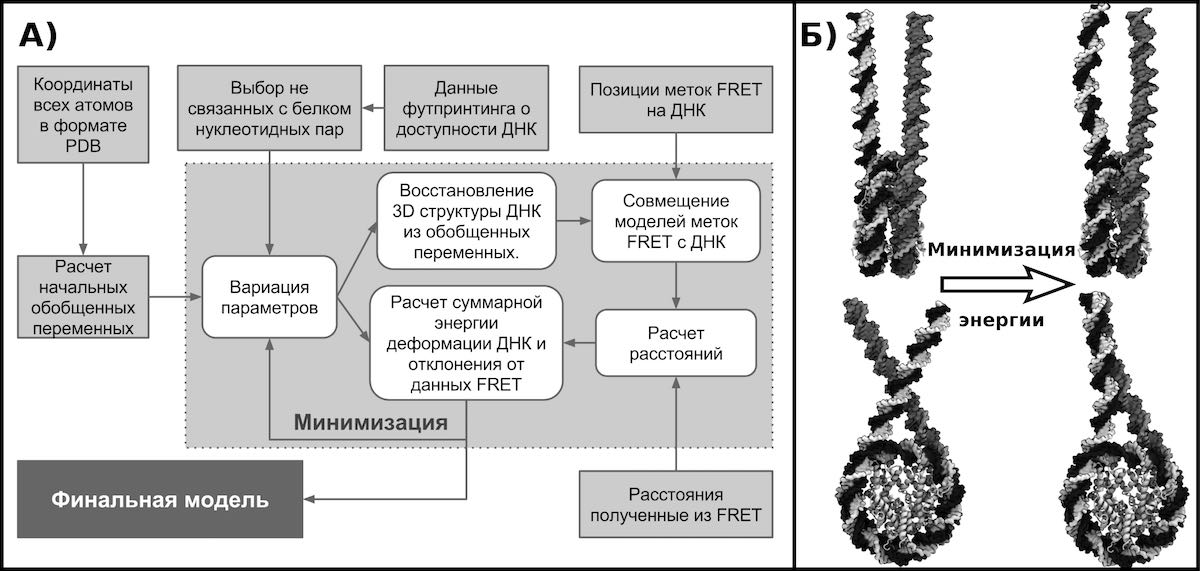
\includegraphics[width=\textwidth]{images/p6/p6_5/p6_5_f2.pdf}
    \caption[Создание моделей ДНК в хроматосоме по данным FRET.]{Создание моделей ДНК в хроматосоме по данным FRET. A) Схема алгоритма поиска конформации ДНК с учетом FRET и дригих данных. Пунктиром выделен блок минимизации энергии при поиске структур. Б) Визуализация результата поиска конформации хроматосомы. Гистоны отображены в виде вторичной структуры, ДНК показана в поверхности доступной растворителю.
}
    \label{fig:p6_5_f2}
\end{figure}

К недостаткам такого подхода можно отнести отсутствие учета взаимодействий между участками ДНК, что может привести к возникновению стерических перекрываний внутри молекулы. Однако при корректном выборе участков ДНК для минимизации, появление таких структур маловероятно.
В качестве объекта для испытания метода была использована нуклеосома с гистоном H1. Этот комплекс на момент проведения работы отсутствовал в банке трехмерных структур PDB, но были работы, где его структура исследуется при помощи ядерного магнитного резонанса \cite{zhou_structural_2013}. Гистон Н1, также называемый линкерным, образует комплекс с нуклеосомами, способствуя более высокому уровню компактизации ДНК. Оказывая такое влияние на размещение/упорядочение   ДНК в клетке, гистон Н1 играет большую роль в регуляции экспрессии генов. Структурные особенности взаимодействия линкерного гистона и нуклеосомы до сих пор неизвестны и их изучение вызывает большой интерес. 
За основу для построения модели была выбрана структура 1KX5 \cite{davey_solvent_2002} из банка данных PDB к которой были добавлены прямые линкеры в соответствии с последовательностью, что применялась в эксперименте FRET.  После проведения минимизации геометрии ДНК с ограничениями расстояний из данных FRET была получена асимметричная структура с параллельным расположением линкерных участков ДНК. Весьма схожие модели были получены в работе \cite{syed_single-base_2010}, где структуру хроматосом исследовали методом гидроксильного футпринтинга и электронной микроскопии. В дальнейшем полученная структура может быть применена в качестве мишени для макромолекулярного докинга гистона H1. 
Понимание молекулярных основ функционирования хроматина встречается с проблемами ограниченности экспериментальных методик в определении параметров взаимодействий ДНК с гистонами, транскрипционными факторами и структурными белками на молекулярном уровне. Данная проблема является следствием того, что экспериментальные методы вроде РСА, ЯМР и электронной микроскопии в состоянии определить структуры лишь небольших комплексов, которые обладают компактной и упорядоченной структурой. В то же время все больший интерес привлекают к себе структуры, не отличающиеся строгой упорядоченностью и их описание хроматина должно вестись не в рамках одиночных структур, а в рамках набора конформационных ансамблей.
Разработан метод, позволяющий создавать модели геометрии ДНК в комплексах с белками на основании интегрирования экспериментальных данных и данных о локальной жесткости ДНК при помощи молекулярного моделирования. Данный метод позволяет получать атомистические модели, позволяя изучать особенности комплексов как внутри, так и с другими. На примере хроматосомы показана возможность получения геометрии линкерной ДНК, что важно для понимания устройства хроматина. 
\emph{Благодарности}
Авторы работы выражают благодарность проф. В.М. Студитскому, проф. А.В.Феофанову и сотрудникам их лабораторий за предоставленные данные FRET.Данная работа выполнена при поддержке гранта Российского научного фонда (грант N14-24-00031).

\textit{>>}

\section{Выводы главы \ref{part6_nucl_complex}}

Автором продемонстрировано, что методы интегративного моделирования способны решать важный класс задач при изучении супрануклеосомной структуры хроматина, исследования которой затруднительны классическими методами структурной биологии, а именно создавать модели комплексов нуклеосом с белками хроматина на основе использования экспериментальных данных электронной микроскопии низкого разрешения, данных FRET-микроскопии, данных футпринтинга ДНК. Получены структурные и динамические модели различных комплексов, возникающих при взаимодействии нуклеосом с РНК-полимеразами, гистоном H1, комплексом FACT.




% \subsection{Положения выносимые на защиту}
% %положения выносимые на защиту
% \begin{enumerate}
%   \item Развиты методы интегративного моделирования супрануклеосомной структуры хроматина, построены структурные модели нуклеосом в различных конформационных состояниях при взаимодействии с рядом белков хроматина.
 
% \end{enumerate}